\chapter{Background}
This chapter introduces all the background needed for our research into offensive eBPF applications. Although our rootkit has been developed using a library that will provide us with a layer of abstraction over the underlying operations, this background is needed to understand how eBPF is embedded in the kernel and which capabilities and limits we can expect to achieve with it.

Firstly, we will analyse the origins of the eBPF technology, understanding what it is and how it works, and discuss the reasons why it is a necessary component of the Linux kernel today. Afterwards, we will cover the main features of eBPF in detail and discuss the security features incorporated in the system, together with an study of the currently existing alternatives for developing eBPF applications.

Finally, we will offer an overview into multiple aspects of the Linux system (memory, networking and executable files), which will be critical during the design of the offensive techniques incorporated in our rootkit.

\section{BPF}
In this section we will detail the origins of eBPF in the Linux kernel. By offering us background into the earlier versions of the system, the goal is to acquire insight on the design decisions included in modern versions of eBPF.

\subsection{Introduction to the BPF system}
Nowadays eBPF is not officially considered to be an acronym anymore \cite{ebpf_io}, but it remains largely known as "extended Berkeley Packet Filters", given its roots in the Berkeley Packet Filter (BPF) technology, now known as classic BPF.

BPF was introduced in 1992 by Steven McCanne and Van Jacobson in the paper "The BSD Packet Filter: A New Architecture for User-level Packet Capture" \cite{bpf_bsd_origin}, as a new filtering technology for network packets in the BSD platform. It was first integrated in the Linux kernel on version 2.1.75 \cite{ebpf_history_opensource}.


\begin{figure}[htbp]
	\centering
	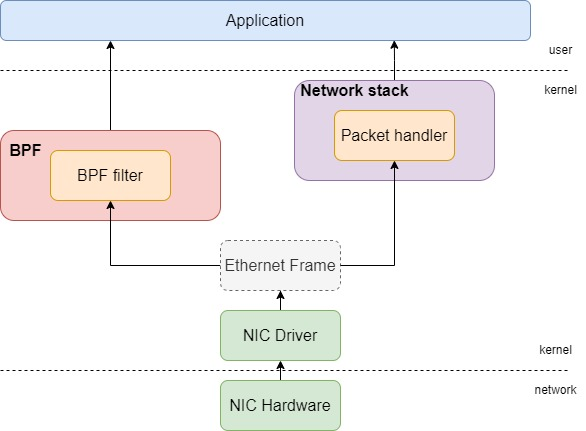
\includegraphics[width=12cm, keepaspectratio=true]{classic_bpf.jpg}
	\caption{Functionality of classic BPF. Based on the figure at the original paper \cite{bpf_bsd_origin_bpf_page2}.}
	\label{fig:classif_bpf}
\end{figure}

Figure \ref{fig:classif_bpf} shows how BPF was integrated in the existing network packet processing by the kernel. After receiving a packet via the Network Interface Controller (NIC) driver, it would first be analysed by BPF filters, which are programs directly developed by the user. This filter decides whether the packet is to be accepted by analysing the packet properties, such as its length or the type and values of its headers. If a packet is accepted, the filter proceeds to decide how many bytes of the original buffer are passed to the application at the user space. Otherwise, the packet is redirected to the original network stack, where it is managed as usual.


\subsection{The BPF virtual machine} \label{subsection:bpf_vm}
In a technical level, BPF comprises both the BPF filter programs developed by the user and the BPF module included in the kernel which allows for loading and running the BPF filters. This BPF module in the kernel works as a virtual machine \cite{bpf_bsd_origin_bpf_page1}, meaning that it parses and interprets the filter program by providing simulated components needed for its execution, turning into a software-based CPU. Because of this reason, it is usually referred as the BPF Virtual Machine (BPF VM). The BPF VM comprises the following components:
\begin{itemize}
\item \textbf{An accumulator register}, used to store intermediate values of operations.
\item \textbf{An index register}, used to modify operand addresses, it is usually incorporated to optimize vector operations \cite{index_register}.
\item \textbf{A scratch memory store}, a temporary storage.
\item \textbf{A program counter}, used to point to the next machine instruction to execute in a filter program.
\end{itemize}


\subsection{Analysis of a BPF filter program} \label{subsection:analysis_bpf_filter_prog}
As we mentioned in Section \ref{subsection:bpf_vm}, the components of the BPF VM are used to support running BPF filter programs. A BPF filter is implemented as a boolean function:
\begin{itemize}
\item If it returns \textit{true}, the kernel copies the packet to the application.
\item If it returns \textit{false}, the packet is not accepted by the filter (and thus the network stack will be the next to operate it).
\end{itemize}

Figure \ref{fig:cbpf_prog} shows an example of a BPF filter upon receiving a packet. In the figure, green lines indicate that the condition is true and red lines that it is evaluated as false. Therefore, the execution works as a control flow graph (CFG) which ends on a boolean value \cite{bpf_bsd_origin_bpf_page5}. The figure presents an example BPF program which accepts the following frames:
\begin{itemize}
\item Frames with an IP packet as a payload directed from IP address X.
\item Frames with an IP packet as a payload directed towards IP address Y.
\item Frames belonging to the ARP protocol and from IP address Y.
\item Frames not from the ARP protocol directed from IP address Y to IP address X.
\end{itemize}

\begin{figure}[ht]
	\centering
	\includegraphics[width=8cm]{cbpf_prog.jpg}
	\caption{Execution of a BPF filter.}
	\label{fig:cbpf_prog}
\end{figure}


\subsection{BPF bytecode instruction format}
In order to implement the CFG to be run at the BPF VM, BPF filter programs are made up of BPF bytecode, which is defined by a new BPF instruction set. Therefore, a BPF filter program is an array of BPF bytecode instructions \cite{bpf_organicprogrammer_analysis}.


\begin{table}[htbp]
\begin{tabular}{|c|c|c|c|c|}
\hline
& \textbf{OPCODE} & \textbf{JT} & \textbf{JF} & \textbf{K}\\
\hline
\textbf{BITS} & 16 & 8 & 8 & 32\\
\hline
\end{tabular}
\caption{BPF instruction format.}
\label{table:bpf_inst_format}
\end{table}

Table \ref{table:bpf_inst_format} shows the format of a BPF bytecode instruction. As it can be observed, it is a fixed-length 64-bit instruction composed of:
\begin{itemize}
\item An \textbf{opcode}, similar to assembly opcode, it indicates the operation to be executed.
\item Field \textbf{jt} indicates the offset to the next instruction to jump in case a condition is evaluated as \textit{true}.
\item Field \textbf{jf} indicates the offset to the next instruction to jump in case a condition is evaluated as \textit{false}.
\item Field \textbf{k} is miscellaneous and its contents vary depending on the instruction opcode.
\end{itemize}

Figure \ref{fig:bpf_instructions} shows how BPF instructions are defined according to the BPF instruction set. As we mentioned, similarly to assembly, instructions include an opcode which indicates the operation to execute, and the multiple arguments defining the arguments of the operation. The table shows, in order by rows, the following instruction types \cite{bpf_bsd_origin_bpf_page8}:
\begin{itemize}
\item Rows 1-4 are \textbf{load instructions}, copying the addressed value into the index or accumulator register.
\item Rows 4-6 are \textbf{store instructions}, copying the accumulator or index register into the scratch memory store.
\item Rows 7-11 are \textbf{jump instructions}, changing the program counter register. These are usually present on each node of the CFG and evaluate whether the condition to be evaluated is true or not.
\item Rows 12-19 and 21-22 are \textbf{arithmetic and miscellaneous instructions}, performing operations usually needed during the program execution.
\item Row 20 is a \textbf{return instruction}, it is positioned in the final end of the CFG, and indicate whether the filter accepts the packet (returning true) or otherwise rejects it (return false).
\end{itemize}

\begin{figure}[htbp]
	\centering
	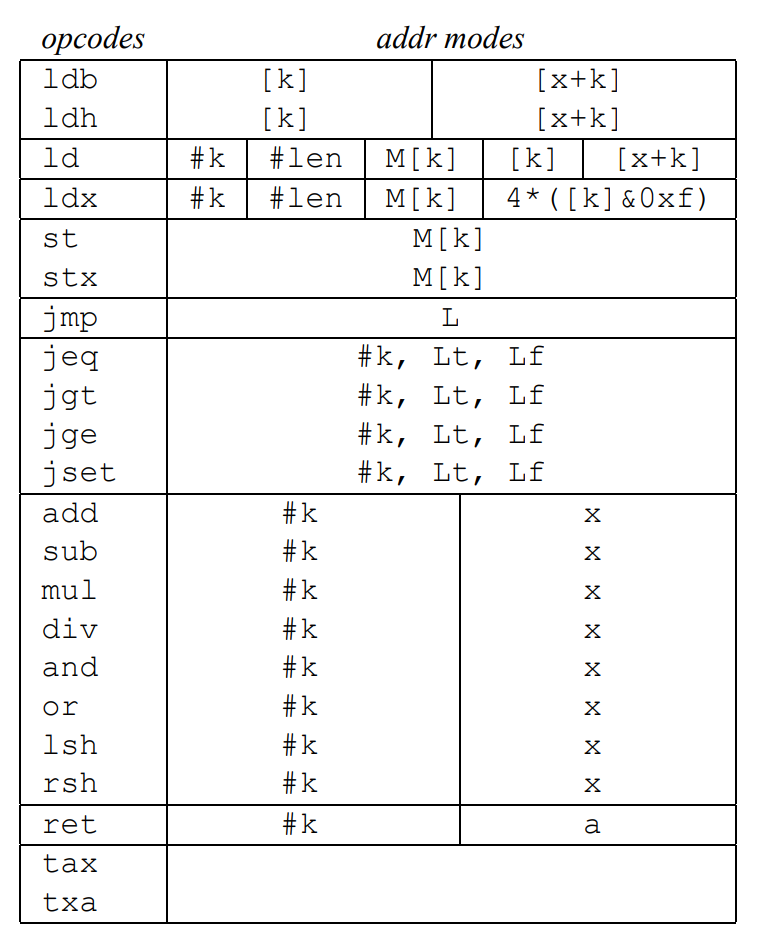
\includegraphics[width=8cm]{bpf_instructions.png}
	\caption{Supported classic BPF instructions, as shown by McCanne and Jacobson \cite{bpf_bsd_origin_bpf_page7}}
	\label{fig:bpf_instructions}
\end{figure}

The column \textit{addr modes} in Figure \ref{fig:bpf_instructions} describes how the parameters of a BPF instruction are referenced depending on the opcode. The address modes are detailed in Figure \ref{fig:bpf_address_mode}. As it can be observed, parameters may consist of immediate values, offsets to memory positions or on the packet, the index register or combinations of the previous.

\begin{figure}[htbp]
	\centering
	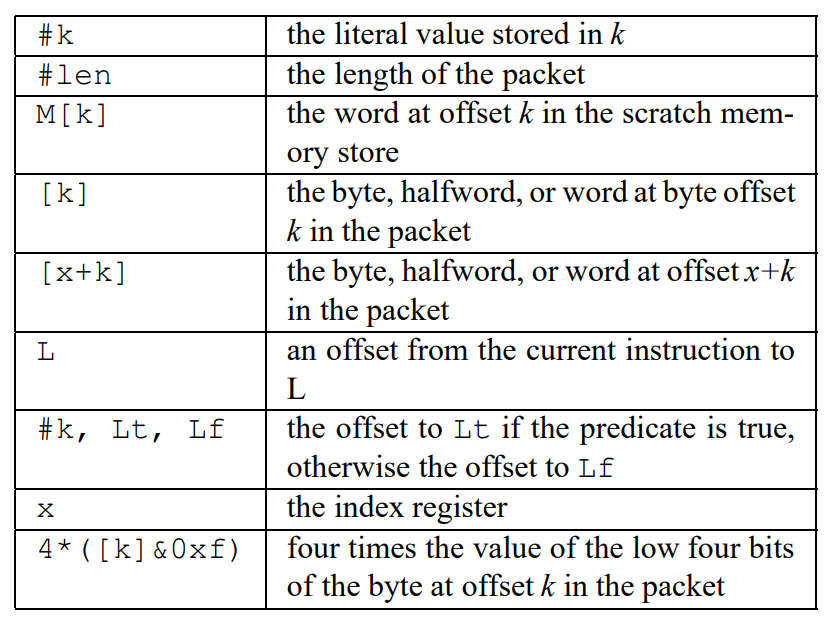
\includegraphics[width=8cm]{bpf_address_mode.png}
	\caption{BPF address modes, as shown by McCanne and Jacobson \cite{bpf_bsd_origin_bpf_page8}}
	\label{fig:bpf_address_mode}
\end{figure}

\subsection{An example of BPF filter with tcpdump} \label{subsection:tcpdump}
At the time, by filtering packets before they are handled by the kernel instead of using a user-level application, BPF offered a performance improvement between 10 and 150 times the state-of-the art technologies of the moment \cite{bpf_bsd_origin_bpf_page1}. Since then, multiple popular tools began to use BPF, such as the network tracing tool \textit{tcpdump} \cite{tcpdump_page}.

\textit{tcpdump} is a command-line tool that enables to capture and analyse the network traffic going through the system. It works by setting filters on a network interface, so that it shows the packets that are accepted by the filter. Still today, \textit{tcpdump} uses BPF for the filter implementation. Figure \ref{fig:bpf_tcpdump_example} shows an example of BPF code used by \textit{tcpdump} to implement a simple filter.

\begin{figure}[htbp]
	\centering
	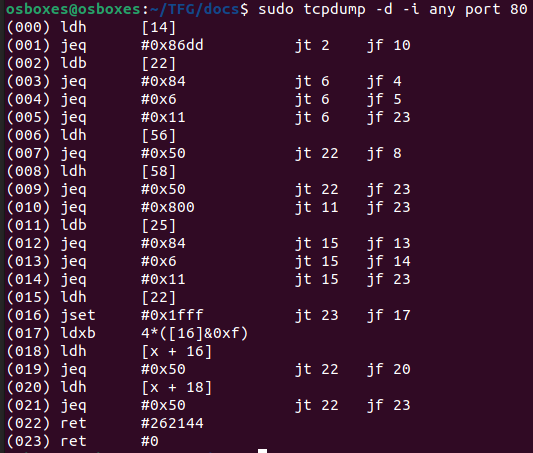
\includegraphics[width=10cm]{tcpdump_example.png}
	\caption{BPF bytecode tcpdump needs to set a filter to display packets directed to port 80.}
	\label{fig:bpf_tcpdump_example}
\end{figure}

In Figure \ref{fig:bpf_tcpdump_example} we can see how tcpdump sets a filter to display traffic directed to all interfaces (\textit{-i any}) directed to port 80. Flag \textit{-d} instructs tcpdump to display BPF bytecode.

In the example, using the \textit{jf} and \textit{jt} fields, we can label the nodes of the CFG described by the BPF filter. Figure \ref{fig:tcpdump_ex_sol} describes the shortest graph path that a true comparison will need to follow to be accepted by the filter. Note how instruction 010 is checking the value 80, the one our filter is looking for in the port.

\begin{figure}[htbp]
	\centering
	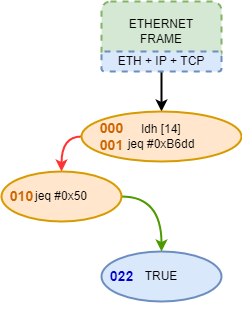
\includegraphics[width=6cm]{cBPF_prog_ex_sol.png}
	\caption{Shortest path in the CFG described in the code shown in Figure \ref{fig:bpf_tcpdump_example} that a packet needs to follow to be accepted by the BPF filter.}
	\label{fig:tcpdump_ex_sol}
\end{figure}

\section{Modern eBPF} \label{section:modern_ebpf}
This section discusses the current state of eBPF in the Linux kernel. By building on the previous architecture described in classic BPF, we will be able to provide a comprehensive picture of the underlying infrastructure in which eBPF relies today.

The addition of classic BPF in the Linux kernel set the foundations of eBPF, but nowadays it has already extended its presence to many other components other than traffic filtering. Similarly to how BPF filters were included in the networking module of the Linux kernel, we will now study the necessary changes made in the kernel to support these new program types. Table \ref{table:ebpf_history} shows the main updates that were incorporated and shaped modern eBPF of today.

\begin{table}[htbp]
\begin{tabular}{|c|c|c|}
\hline
\textbf{DESCRIPTION} & \textbf{KERNEL VERSION} & \textbf{YEAR}\\
\hline
\hline
\textit{BPF}: First addition in the kernel & 2.1.75 & 1997\\
\textit{BPF+}: New JIT assembler & 3.0 & 2011\\
\textit{eBPF}: Added eBPF support & 3.15 & 2014\\
\textit New bpf() syscall & 3.18 & 2014\\
\textit Introduction of eBPF maps & 3.19 & 2015\\
\textit eBPF attached to kprobes & 4.1 & 2015\\
\textit Introduction of Traffic Control & 4.5 & 2016\\
\textit eBPF attached to tracepoints & 4.7 & 2016\\
\textit Introduction of XDP & 4.8 & 2016\\


\hline
\end{tabular}
\caption{Relevant eBPF updates. Selection of the official complete table at \cite{ebpf_funcs_by_ver}.}
\label{table:ebpf_history}
\end{table}

As it can be observed in the table above, the main breakthrough happened in the 3.15 version, where Alexei Starovoitov, along with Daniel Borkmann, decided to expand the capabilities of BPF by remodelling the BPF instruction set and overall architecture \cite{brendan_gregg_bpf_book}.

Figure \ref{fig:ebpf_architecture} offers an overview of the current eBPF architecture. During the subsequent subsections, we will proceed to explain its components in detail.

\begin{figure}[htbp]
	\centering
	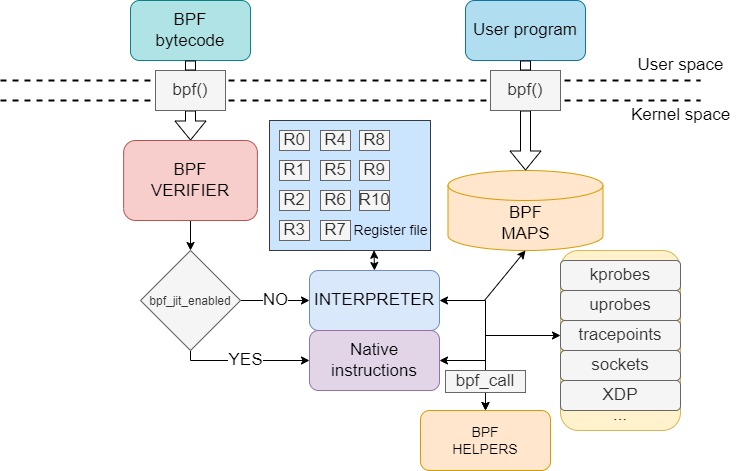
\includegraphics[width=15cm]{ebpf_arch.jpg}
	\caption{eBPF architecture in the Linux kernel and the process of loading an eBPF program. Based on \cite{brendan_gregg_bpf_book} and \cite{ebpf_io_arch}.}
	\label{fig:ebpf_architecture}
\end{figure}

\subsection{eBPF instruction set} \label{subsection:ebpf_inst_set}
The eBPF update included a complete remodel of the instruction set architecture (ISA) of the BPF VM. Therefore, eBPF programs will need to follow the new architecture in order to be interpreted as valid and executed.

Table \ref{table:ebpf_inst_format} shows the new instruction format for eBPF programs \cite{ebpf_inst_set}. As it can be observed, it is a fixed-length 64-bit instruction. The new fields are similar to x86\_64 assembly, incorporating the typically found immediate and offset fields, and source and destination registers \cite{8664_inst_set_specs}. Similarly, the instruction set is extended to be similar to the one typically found on x86\_64 systems, the complete list can be consulted in the official documentation \cite{ebpf_inst_set}.
%Should I talk about assembly or this more in detail?

\begin{table}[htbp]
\begin{tabular}{|c|c|c|c|c|c|}
\hline
& \textbf{IMM} & \textbf{OFF} & \textbf{SRC} & \textbf{DST} & \textbf{OPCODE} \\
\hline
\textbf{BITS} & 32 & 16 & 4 & 4 & 8\\
\hline
\end{tabular}
\caption{eBPF instruction format.}
\label{table:ebpf_inst_format}
\end{table}

With respect to the BPF VM registers, they get extended from 32 to 64 bits of length, and the number of registers is incremented to 10, instead of the original accumulator and index registers. These registers are also adapted to be similar to those in assembly, as it is shown in Table \ref{table:ebpf_regs}.

\begin{table}[htbp]
\begin{tabular}{|>{\centering\arraybackslash}p{2.5cm}|>{\centering\arraybackslash}p{2.5cm}|>{\centering\arraybackslash}p{7cm}|}
\hline
\textbf{eBPF REGISTER} & \textbf{x86\_64 REGISTER} & \textbf{PURPOSE}\\
\hline
\hline
r0 & rax & Return value from functions and exit value of eBPF programs\\
\hline
r1 & rdi & Function call argument 1\\
\hline
r2 & rsi & Function call argument 2\\
\hline
r3 & rdx & Function call argument 3\\
\hline
r4 & rcx & Function call argument 4\\
\hline
r5 & r8 & Function call argument 5\\
\hline
r6 & rbx & Callee saved register, value preserved between calls\\
\hline
r7 & r13 & Callee saved register, value preserved between calls\\
\hline
r8 & r14 & Callee saved register, value preserved between calls\\
\hline
r9 & r15 & Callee saved register, value preserved between calls\\
\hline
r10 & rbp & Frame pointer for stack, read only\\
\hline
\end{tabular}
\caption{eBPF registers and their purpose in the BPF VM. \cite{ebpf_inst_set} \cite{ebpf_starovo_slides}.}
\label{table:ebpf_regs}
\end{table}

\subsection{JIT compilation}
We mentioned in Section \ref{subsection:ebpf_inst_set} that eBPF registers and instructions describe an almost one-to-one correspondence to those in x86 assembly. This is in fact not a coincidence, but rather it is with the purpose of improving a functionality that was included in Linux kernel 3.0, called Just-in-Time (JIT) compilation \cite{ebpf_JIT} \cite{ebpf_JIT_demystify_page13}.

JIT compiling is an extra step that optimizes the execution speed of eBPF programs. It consists of translating BPF bytecode into machine-specific instructions, so that they run as fast as native code in the kernel. Machine instructions are generated during runtime, written directly into executable memory and executed there \cite{ebpf_JIT_demystify_page14}.

Therefore, when using JIT compiling (a setting defined by the variable \textit{bpf\_jit\_enable} \cite{jit_enable_setting}, BPF registers are translated into machine-specific registers following their one-to-one mapping and bytecode instructions are translated into machine-specific instructions \cite{ebpf_starovo_slides_page23}. There no longer exists an interpretation step by the BPF VM, since we can execute the code directly \cite{brendan_gregg_bpf_book_bpf_vm}.

The programs developed during this project will always have JIT compiling active.


\subsection{The eBPF verifier} \label{subsection:ebpf_verifier}
We introduced in Figure \ref{fig:ebpf_architecture} the presence of the so-called eBPF verifier. Provided that we will be loading programs in the kernel from user space, these programs need to be checked for safety before being valid to be executed.

The verifier performs a series of tests which every eBPF program must pass in order to be accepted. Otherwise, user programs could leak privileged data, result in kernel memory corruption, or hang the kernel in an infinite loop, between others. Therefore, the verifier limits multiple aspects of eBPF programs so that they are restricted to the intended functionality, whilst at the same time offering a reasonable amount of freedom to the developer.

The following are the most relevant checks that the verifier performs in eBPF programs \cite{ebpf_verifier_kerneldocs} \cite{ebpf_JIT_demystify_page17-22}:
\begin{itemize}
\item Tests for ensuring overall control flow safety:
	\subitem No loops allowed (bounded loops accepted since kernel version 5.3 \cite{ebpf_bounded_loops}.
	\subitem Function call and jumps safety to known, reachable functions.
	\subitem Sleep and blocking operations not allowed (to prevent hanging the kernel).
\item Tests for individual instructions:
	 \subitem Divisions by zero and invalid shift operations.
	 \subitem Invalid stack access and invalid out-of-bound access to data structures.
	 \subitem Reads from uninitialized registers and corruption of pointers.
\end{itemize}

These checks are performed by two main algorithms:
\begin{itemize}
\item Build a graph representing the eBPF instructions (similar to the one shown in Section \ref{subsection:analysis_bpf_filter_prog}. Check that it is in fact a direct acyclic graph (DAG), meaning that the verifier prevents loops and unreachable instructions.
\item Simulate execution flow by starting on the first instruction and following each possible path, observing at each instruction the state of every register and of the stack.
\end{itemize}

\subsection{eBPF maps} \label{subsection:ebpf_maps}
An eBPF map is a generic storage for eBPF programs used to share data between user and kernel space, to maintain persistent data between eBPF calls and to share information between multiple eBPF programs \cite{ebpf_maps_kernel}.

A map consists of a key + value tuple. Both fields can have an arbitrary data type, the map only needs to know the length of the key and the value field at its creation \cite{bpf_syscall}. Programs can open maps by specifying their ID, and lookup or delete elements in the map by specifying its key, also insert new ones by supplying the element value and they key to store it with.

Therefore, creating a map requires a struct with the fields shown in Table \ref{table:ebpf_map_struct}.

\begin{table}[htbp]
\begin{tabular}{|c|c|}
\hline
\textbf{FIELD} & \textbf{VALUE}\\
\hline
\hline
type & Type of eBPF map. Described in Table \ref{table:ebpf_map_types}\\
\hline
key\_size & Size of the data structure to use as a key\\
\hline
value\_size & Size of the data structure to use as value field\\
\hline
max\_entries & Maximum number of elements in the map\\
\hline
\end{tabular}
\caption{Common fields for creating an eBPF map.}
\label{table:ebpf_map_struct}
\end{table}

Table \ref{table:ebpf_map_types} describes the main types of eBPF maps that are available for use. During the development of our rootkit, we will mainly focus on hash maps (BPF\_MAP\_TYPE\_HASH), provided that they are simple to use and we do not require of any special storage for our research purposes.

\begin{table}[htbp]
\begin{tabular}{|c|>{\centering\arraybackslash}p{7cm}|}
\hline
\textbf{TYPE} & \textbf{DESCRIPTION}\\
\hline
\hline
BPF\_MAP\_TYPE\_HASH & A hast table-like storage, elements are stored in tuples.\\
\hline
BPF\_MAP\_TYPE\_ARRAY & Elements are stored in an array.\\
\hline
BPF\_MAP\_TYPE\_RINGBUF & Map providing alerts from kernel to user space, covered in Section \ref{subsection:bpf_ring_buf}\\
\hline
BPF\_MAP\_TYPE\_PROG\_ARRAY & Stores descriptors of eBPF programs\\
\hline
\hline
\end{tabular}
\caption{Relevant types of eBPF maps. Full list can be consulted in the man page \cite{bpf_syscall}}
\label{table:ebpf_map_types}
\end{table}

\subsection{The eBPF ring buffer} \label{subsection:bpf_ring_buf}
eBPF ring buffers are a special kind of eBPF maps, providing a one-way directional communication system, going from an eBPF program in the kernel to a user space program that subscribes to its events.

%TODO DIAGRAM OF A TYPICAL RING BUFFER

\subsection{The bpf() syscall} \label{subsection:bpf_syscall}
The bpf() syscall is used to issue commands from user space to kernel space in eBPF programs. This syscall is multiplexor, meaning that it can perform a great range of actions, changing its behaviour depending on the parameters.

The main operations that can be issued are described in Table \ref{table:ebpf_syscall}:

\begin{table}[htbp]
\begin{tabular}{|c|>{\centering\arraybackslash}p{4cm}|>{\centering\arraybackslash}p{4cm}|}
\hline
\textbf{COMMAND} & \textbf{ATTRIBUTES} & \textbf{DESCRIPTION}\\
\hline
\hline
BPF\_MAP\_CREATE & Struct with map info as defined in Table \ref{table:ebpf_map_struct} & Create a new map\\
\hline
BPF\_MAP\_LOOKUP\_ELEM & Map ID, and struct with key to search in the map & Get the element on the map with a specific key\\
\hline
BPF\_MAP\_UPDATE\_ELEM & Map ID, and struct with key and new value & Update the element of an specific key with a new value\\
\hline
BPF\_MAP\_DELETE\_ELEM & Map ID and struct with key to search in the map & Delete the element on the map with an specific key\\
\hline
BPF\_PROG\_LOAD & Struct describing the type of eBPF program to load & Load an eBPF program in the kernel\\
\hline
\end{tabular}
\caption{Relevant types of syscall actions. Full list and attribute details can be consulted in the man page \cite{bpf_syscall}}
\label{table:ebpf_syscall}
\end{table}

With respect to the program type indicated with BPF\_PROG\_LOAD, this parameter indicates the type of eBPF program, setting the context in the kernel in which it will run, and to which modules it will have access to. The types of programs relevant for our research are described in Table \ref{table:ebpf_prog_types}.

\begin{table}[htbp]
\begin{tabular}{|c|>{\centering\arraybackslash}p{5cm}|}
\hline
\textbf{PROGRAM TYPE} & \textbf{DESCRIPTION}\\
\hline
\hline
BPF\_PROG\_TYPE\_KPROBE & Program to instrument code to an attached kprobe\\
\hline
BPF\_PROG\_TYPE\_UPROBE & Program to instrument code to an attached uprobe\\
\hline
BPF\_PROG\_TYPE\_TRACEPOINT & Program to instrument code to a syscall tracepoint\\
\hline
BPF\_PROG\_TYPE\_XDP & Program to filter, redirect and monitor network events from the Xpress Data Path\\
\hline
BPF\_PROG\_TYPE\_SCHED\_CLS & Program to filter, redirect and monitor events using the Traffic Control classifier\\
\hline
\end{tabular}
\caption{Relevant types of eBPF programs. Full list and attribute details can be consulted in the man page \cite{bpf_syscall}.}
\label{table:ebpf_prog_types}
\end{table}

In Section \ref{section:ebpf_prog_types}, we will proceed to analyse in detail the different program types and what capabilities they offer.

\subsection{eBPF helpers} \label{subsection:ebpf_helpers}
Our last component to cover of the eBPF architecture are the eBPF helpers. Since eBPF programs have limited accessibility to kernel functions (which kernel modules commonly have free access to), the eBPF system offers a set of limited functions called helpers \cite{ebpf_helpers}, which are used by eBPF programs to perform certain actions and interact with the context on which they are run. The list of helpers a program can call varies between eBPF program types, since different programs run in different contexts.

It is important to highlight that, just like commands issued via the bpf() syscall can only be issued from the user space, eBPF helpers correspond to the kernel-side of eBPF program exclusively. Note that we will also find a symmetric correspondence to those functions of the bpf() syscall related to map operations (since these are accessible both from user and kernel space).

Table \ref{table:ebpf_helpers} lists the most relevant general-purpose eBPF helpers we will use during the development of our project. We will later detail those helpers exclusive to an specific eBPF program type in the sections on which they are studied.

\begin{table}[htbp]
\begin{tabular}{|c|>{\centering\arraybackslash}p{8cm}|}
\hline
\textbf{eBPF HELPER}& \textbf{DESCRIPTION}\\
\hline
\hline
bpf\_map\_lookup\_elem() & Query an element with a certain key in a map\\
\hline
bpf\_map\_delete\_elem() & Delete an element with a certain key in a map\\
\hline
bpf\_map\_update\_elem() & Update the value of the element with a certain key in a map\\
\hline
bpf\_probe\_read\_user() & Attempt to safely read data at an specific user address into a buffer\\
\hline
bpf\_probe\_read\_kernel() & Attempt to safely read data at an specific kernel address into a buffer\\
\hline
bpf\_trace\_printk() & Similarly to printk() in kernel modules, writes buffer in \/sys\/kernel\/debug\/tracing\/trace\_pipe\\
\hline
bpf\_get\_current\_pid\_tgid() & Get the process' Process Id (PID) and thread group id (TGID)\\
\hline
bpf\_get\_current\_comm() & Get the name of the executable\\
\hline
bpf\_probe\_write\_user() & Attempt to write data at a user memory address\\
\hline
bpf\_override\_return() & Override return value of a probed function\\
\hline
bpf\_ringbuf\_submit() & Submit data to an specific eBPF ring buffer, and notify to subscribers\\
\hline
bpf\_tail\_call() & Jump to another eBPF program preserving the current stack\\
\hline
\end{tabular}
\caption{Relevant common eBPF helpers. Helpers exclusive to an specific program type are not listed. Full list and attribute details can be consulted in the man page \cite{ebpf_helpers}.}
\label{table:ebpf_helpers}
\end{table}


\section{eBPF program types} \label{section:ebpf_prog_types}
In the previous subsection \ref{subsection:bpf_syscall} we introduced the new types of eBPF programs that are supported and that we will be developing for our offensive analysis. In this section, we will analyse in greater detail how eBPF is integrated in the Linux kernel in order to support these new functionalities.

\subsection{XDP} \label{subsection:xdp}
Express Data Path (XDP) programs are a novel type of eBPF program that allows for the lowest-latency traffic filtering and monitoring in the whole Linux kernel. In order to load an XDP program, a bpf() syscall with the command BPF\_PROG\_LOAD and the program type BPF\_PROG\_TYPE\_XDP must be issued. 

These programs are directly attached to the Network Interface Controller (NIC) driver, and thus they can process the packet before any other module \cite{xdp_gentle_intro}.

Figure \ref{fig:xdp_diag} shows how XDP is integrated in the network processing of the Linux kernel. After receiving a raw packet (in the figure, \textit{xdp\_md}, which consists on the raw bytes plus some very basic metadata about the packet) from the incoming traffic, XDP program can perform the following actions \cite{xdp_manual}:
\begin{itemize}
\item Analyse the data between the packet buffer bounds.
\item Modify the packet contents, and modify the packet length.
\item Decide between one of the actions displayed in Table \ref{table:xdp_actions_av}.
\end{itemize}

\begin{figure}[htbp]
	\centering
	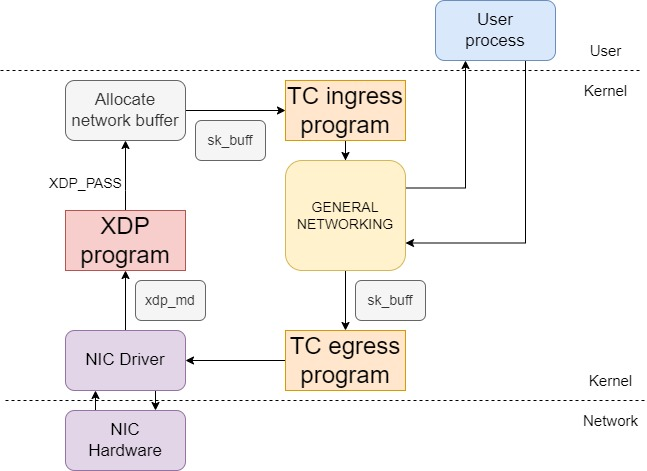
\includegraphics[width=15cm]{xdp_diag.jpg}
	% Either this caption, or change the text afterwards. I still need to know whether to put the long explanation here or on the paragraph, it gets repetitive.
	\caption{XDP and TC modules integration in the network processing module of the Linux kernel.}
	\label{fig:xdp_diag}
\end{figure}

\begin{table}[htbp]
\begin{tabular}{|c|>{\centering\arraybackslash}p{10cm}|}
\hline
\textbf{ACTION} & \textbf{DESCRIPTION}\\
\hline
\hline
XDP\_PASS & Let packet proceed with operated modifications on it.\\
\hline
XDP\_TX & Return the packet at the same NIC it was received from. Packet modifications are kept.\\
\hline
XDP\_DROP & Drops the packet completely, kernel networking will not be notified.\\
\hline
\end{tabular}
\caption{Relevant XDP return values.}
\label{table:xdp_actions_av}
\end{table}

Some of the XDP-exclusive eBPF helpers we will be discussing in later sections are shown in Table \ref{table:xdp_helpers}.
\begin{table}[htbp]
\begin{tabular}{|c|>{\centering\arraybackslash}p{8cm}|}
\hline
\textbf{eBPF HELPER} & \textbf{DESCRIPTION}\\
\hline
\hline
bpf\_xdp\_adjust\_head() & Enlarges or reduces the extension of a packet, by moving the address of its first byte.\\
\hline
bpf\_xdp\_adjust\_tail() & Enlarges or reduces the extension of a packet, by moving the address of its last byte.\\
\hline
\end{tabular}
\caption{Relevant XDP-exclusive eBPF helpers.}
\label{table:xdp_helpers}
\end{table}


\subsection{Traffic Control} \label{subsection:tc}
Traffic Control (TC) programs are also indicated for networking instrumentation. Similarly to XDP, their module is positioned before entering the overall network processing of the kernel. However, as it can be observed in Figure \ref{fig:xdp_diag}, they differ in some aspects:
\begin{itemize}
\item TC programs receive a network buffer with metadata (in the figure, \textit{sk\_buff}) about the packet in it. This renders TC programs less ideal than XDP for performing large packet modifications (like new headers), but at the same time the additional metadata fields make it easier to locate and modify specific packet fields \cite{tc_differences}.
\item TC programs can be attached to the \textit{ingress} or \textit{egress} points, meaning that an eBPF program can operate not only over incoming traffic, but also over the outgoing packets.
\end{itemize}

With respect to how TC programs operate, the Traffic Control system in Linux is greatly complex and would require a complete section by itself. In fact, it was already a complete system before the appearance of eBPF. Full documentation can be found at \cite{tc_docs_complete}. For this document, we will explain the overall process needed to load a TC program \cite{tc_direct_action}:
\begin{enumerate}
\item The TC program defines a so-called queuing discipline (qdisc), a packet scheduler that issues packets in a First-In-First-Out (FIFO) order as soon as they are received. This qdisc will be attached to a specific network interface (e.g.: wlan0).
\item Our TC eBPF program is attached to the qdisc. It will work as a filter, being run for every of the packets dispatched by the qdisc.
\end{enumerate}

Similarly to XDP, the TC eBPF programs can decide an action to be executed on a packet by specifying a return value. These actions are almost analogous to the ones in XDP, as it can be observed in Table \ref{table:tc_actions}.

\begin{table}[htbp]
\begin{tabular}{|c|>{\centering\arraybackslash}p{9cm}|}
\hline
\textbf{ACTION} & \textbf{DESCRIPTION}\\
\hline
\hline
TC\_ACT\_OK & Let packet proceed with operated modifications on it.\\
\hline
TC\_ACT\_RECLASSIFY & Return the packet to the back of the qdisc scheduling queue.\\
\hline
TC\_ACT\_SHOT & Drops the packet completely, kernel networking will not be notified.\\
\hline
\end{tabular}
\caption{Relevant TC return values. Full list can be consulted at \cite{tc_ret_list_complete}.}
\label{table:tc_actions}
\end{table}

Finally, as in XDP, there exists a list of useful BPF helpers that will be relevant for the creation of our rootkit. They are shown in Table \ref{table:tc_helpers}.
\begin{table}[htbp]
\begin{tabular}{|c|>{\centering\arraybackslash}p{9cm}|}
\hline
\textbf{eBPF HELPER} & \textbf{DESCRIPTION}\\
\hline
\hline
bpf\_l3\_csum\_replace() & Recomputes the network layer 3 (e.g.: IP) checksum of the packet.\\
\hline
bpf\_l4\_csum\_replace() & Recomputes the network layer 4 (e.g.: TCP) checksum of the packet.\\
\hline
bpf\_skb\_store\_bytes() & Write a data buffer into the packet.\\
\hline
bpf\_skb\_pull\_data() & Reads a sequence of packet bytes into a buffer.\\
\hline
bpf\_skb\_change\_head() & (Only) enlarges the extension of a packet, by moving the address of its first byte.\\
\hline
bpf\_skb\_change\_tail() & Enlarges or reduces the extension of a packet, by moving the address of its last byte.\\
\hline
\hline
\end{tabular}
\caption{Relevant TC-exclusive eBPF helpers.}
\label{table:tc_helpers}
\end{table}


%TODO This section might benefit from some diagrams, maybe. It was a bit to extense already, so skipping it from now
\subsection{Tracepoints} \label{subsection:tracepoints}
Tracepoints are a technology in the Linux kernel that allows to hook functions in the kernel, connecting a 'probe': a function that is executed every time the hooked function is called \cite{tp_kernel}. These tracepoints are set statically during kernel development, meaning that for a function to be hooked, it needs to have been previously marked with a tracepoint statement indicating its traceability. At the same time, this limits the number of tracepoints available.

The list of tracepoint events available depends on the kernel version and can be visited under the directory \textit{/sys/kernel/debug/tracing/events}.

It is particularly relevant for our later research that most of the system calls incorporate a tracepoint, both when they are called (\textit{enter} tracepoint) and when they are exited (\textit{exit} tracepoints). This means that, for a system call sys\_open, both the tracepoint sys\_enter\_open and sys\_exit\_open are available. 

Also, note that the probe functions that are called when hitting a tracepoint receive some parameters related to the context on which the tracepoint is located. In the case of syscalls, these include the parameters with which the syscall was called (only for \textit{enter} syscalls, \textit{exit} ones will only have access to the return value). The exact parameters and their format which a probe function receives can be visited in the file \textit{/sys/kernel/debug/tracing/events/<subsystem>/<tracepoint>/format}. In the previous example with sys\_enter\_open, this is \textit{/sys/kernel/debug/tracing/events/syscalls/sys\_enter\_open/format}.

In eBPF, a program can issue a bpf() syscall with the command BPF\_PROG\_LOAD and the program type BPF\_PROG\_TYPE\_TRACEPOINT, specifying which is the function with the tracepoint to attach to and an arbitrary function probe to call when it is hit. This function probe is defined by the user in the eBPF program submitted to the kernel.

\subsection{Kprobes}
Kprobes are another tracing technology of the Linux kernel whose functionality has been become available to eBPF programs. Similarly to tracepoints, kprobes enable to hook functions in the kernel, with the only difference that it is dynamically attached to any arbitrary function, rather than to a set of predefined positions \cite{kprobe_manual}. It does not require that kernel developers specifically mark a function to be probed, but rather kprobes can be attached to any instruction, with a short list of blacklisted exceptions. 

As it happened with tracepoints, the probe functions have access to the parameters of the original hooked function. Also, the kernel maintains a list of kernel symbols (addresses) which are relevant for tracing and that offer us insight into which functions we can probe. It can be visited under the file \textit{/proc/kallsyms}, which exports symbols of kernel functions and loaded kernel modules \cite{kallsyms_kernel}.

Also similarly, since tracepoints could be found in their \textit{enter} and \textit{exit} variations, kprobes have their counterpart, named kretprobes, which call the hooked probe once a return instruction is reached after the hooked symbol. This means that a kretprobe hooked to a kernel function will call the probe function once it exits.

In eBPF, a program can issue a bpf() syscall with the command BPF\_PROG\_LOAD and the program type BPF\_PROG\_TYPE\_KPROBE, specifying which is the function with the kprobe to attach to and an arbitrary function probe to call when it is hit. This function probe is defined by the user in the eBPF program submitted to the kernel.

\subsection{Uprobes}
Uprobes is the last of the main tracing technologies which has been become accessible to eBPF programs. They are the counterparts of Kprobes, allowing for tracing the execution of an specific instruction in the user space, instead of in the kernel. When the execution flow reaches a hooked instruction, a probe function is run. 

For setting an uprobe on a specific instruction of a program, we need to know three components:
\begin{itemize}
\item The name of the program.
\item The address of the function where the instruction is contained.
\item The offset at which the specific instruction is placed from the start of the function.
\end{itemize}

Similarly to kprobes, uprobes have access to the parameters received by the hooked function. Also, the complementary uretprobes exist too, running the probe function once the hooked function returns.

In eBPF, programs can issue a bpf() syscall with the command BPF\_PROG\_LOAD and the program type BPF\_PROG\_TYPE\_UPROBE, specifying the function with the uprobe to attach to and an arbitrary function probe to call when it is hit. This function probe is also defined by the user in the eBPF program submitted to the kernel.

% Is this the best title?
\section{Developing eBPF programs}
In Section \ref{section:modern_ebpf}, we discussed the overall architecture of the eBPF system which is now an integral part of the Linux kernel. We also studied the process which a piece of eBPF bytecode follows in order to be accepted in the kernel. However, for an eBPF developer, programming bytecode and working with bpf() calls natively is not an easy task, therefore an additional layer of abstraction was needed. 

Nowadays, there exist multiple popular alternatives for writing and running eBPF programs. We will overview which they are and proceed to analyse in further detail the option that we will use for the development of our rootkit.

\subsection{BCC}
BPF Compiler Collection (BCC) is one of the first and well-known toolkits for eBPF programming available \cite{bcc_github}. It allows to include eBPF code into user programs. These programs are developed in Python, and the eBPF code is embedded as a plain string.

Although BCC offers a wide range of tools to easy the development of eBPF programs, we found it not to be the most appropriate for our large-scale eBPF project. In particular, this was due to the feature of eBPF programs being stored as a python string, which leads to difficult scalability, poor development experience given that programming errors are detected at runtime (once the python program issues the compilation of the string), and simply better features from competing libraries.

\subsection{Bpftool}
Bpftool is not a development framework like BCC, but one of the most relevant tools for eBPF program development. Some of its functionalities include:
\begin{itemize}
\item Loading eBPF programs.
\item List running eBPF programs.
\item Dumping bytecode from live eBPF programs.
\item Extract program statistics and data from programs.
\item List and operate over eBPF maps.
\end{itemize}

Although we will not be covering bpftool during our overview on the constructed eBPF rootkit, it was used extensively during the development and became a key tool for debugging eBPF programs, particularly to peek data at eBPF maps during runtime.

\subsection{Libbpf} \label{subsection:libbpf}
Libbpf \cite{libbpf_github} is a library for loading and interacting with eBPF programs, which is currently maintained in the Linux kernel source tree \cite{libbpf_upstream}. It is one of the most popular frameworks to develop eBPF applications, both because it makes eBPF programming similar to common kernel development and because it aims at reducing kernel-version dependencies, thus increasing programs portability between systems \cite{libbpf_core}. During our research, however, we will not make use of this functionalities given that a portable program is not in our research goals.

As we discussed in Section \ref{section:modern_ebpf}, eBPF programs are composed of both the eBPF code in the kernel and a user space program that can interact with it. With libbpf, the eBPF kernel program is developed in C (a real program, not a string later compiled as with BCC), while user programs are usually developed in C, Rust or GO. For our project, we will use the C version of libbpf, so both the user and kernel side of our rootkit will be developed in this language.

% Cites in the following paragraph?
When using libbpf with the C language, both the user-side and kernel eBPF program are compiled together using the Clang/LLVM compiler, translating C instructions into eBPF bytecode. As a clarification, Clang is the front-end of the compiler, translating C instructions into an intermediate form understandable by LLVM, whilst LLVM is the back end compiling the intermediate code into eBPF bytecode. As it can be observed in Figure \ref{fig:libbpf}, the result of the compilation is a single program, comprising the user-side which will launch a user process, the eBPF bytecode to be run in the kernel, and other structures libbpf generates about eBPF maps and other meta data. This program is encapsulated as an ELF file (a common executable format).

\begin{figure}[htbp]
	\centering
	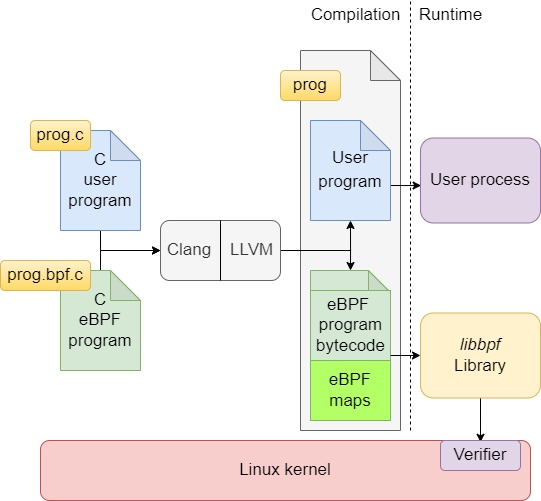
\includegraphics[width=12cm, keepaspectratio=true]{libbpf_prog.jpg}
	\caption{Compilation and loading process of a program developed with libbpf.}
	\label{fig:libbpf}
\end{figure}

Finally, we will overview one of the main functionalities of libbpf to simplify eBPF programming, namely the BPF skeleton. This is auto-generated code by libbpf whose aim is to simplify working with eBPF from the user-side program. As a summary, it parses the eBPF programs developed (which may be using different technologies such as XDP, kprobes, TC...) and the eBPF maps used, and as a result offers a simple set of functions for dealing with these programs from the user program. In particular, it allows for loading and unloading a specific eBPF program from user space at runtime.

Table \ref{table:libbpf_skel} describes the API offered by the BPF skeleton. Note that <name> is substituted by the name of the program being compiled.

\begin{table}[htbp]
\begin{tabular}{|c|>{\centering\arraybackslash}p{9cm}|}
\hline
\textbf{FUNCTION NAME} & \textbf{DESCRIPTION}\\
\hline
\hline
<name>\_\_open() & Parse the eBPF programs and maps.\\
\hline
<name>\_\_load() & Load the eBPF map in the kernel after its validation, create the maps. However, the programs are not active yet.\\
\hline
<name>\_\_attach() & Activate the eBPF programs, attaching them to their corresponding parts in the kernel (e.g. kprobes to kernel functions).\\
\hline
<name>\_\_destroy() & Detach and unload the eBPF programs from the kernel.\\
\hline
\end{tabular}
\caption{BPF skeleton functions.}
\label{table:libbpf_skel}
\end{table}

Note that the BPF skeleton also offers further granularity at the time of dealing with programs, so that individual programs can be loaded or attached instead of all simultaneously. This is the approach we will generally use in the development of our rootkit, as it will be explained in Section \ref{subsection:ebpf_progs_config}.



\section{Security features in eBPF} \label{section:ebpf_security}
As we have shown in Section \ref{section:modern_ebpf}, eBPF has been an active part of the Linux kernel from its 3.18 version. However, as with many other components of the kernel, its availability to the user depends on the parameters with which the kernel has been compiled. Specifically, eBPF is only available to kernels compiled with the flags specified in Table \ref{table:ebpf_kernel_flags}.

\begin{table}[htbp]
\begin{tabular}{|c|c|>{\centering\arraybackslash}p{7cm}|}
\hline
\textbf{FLAG} & \textbf{VALUE} & \textbf{DESCRIPTION}\\
\hline
\hline
\multicolumn{1}{|c|}{CONFIG\_BPF} & \multicolumn{1}{c|}{y} & \multirow{2}{*}{Basic BPF compilation (mandatory)}\\
\cline{1-2}
\multicolumn{1}{|c|}{CONFIG\_BPF\_SYSCALL} & \multicolumn{1}{c|}{m} & \\
\hline
\multicolumn{1}{|c|}{CONFIG\_NET\_ACT\_BPF} & \multicolumn{1}{c|}{m} & \multirow{2}{*}{Traffic Control functionality}\\
\cline{1-2}
\multicolumn{1}{|c|}{CONFIG\_NET\_CLS\_BPF} & \multicolumn{1}{c|}{y} & \\
\hline
\multicolumn{1}{|c|}{CONFIG\_BPF\_JIT} & \multicolumn{1}{c|}{y} & \multirow{2}{*}{Enable JIT compliation}\\
\cline{1-2}
\multicolumn{1}{|c|}{CONFIG\_HAVE\_BPF\_JIT} & \multicolumn{1}{c|}{y} & \\
\hline
\multicolumn{1}{|c|}{CONFIG\_BPF\_EVENTS} & \multicolumn{1}{c|}{y} & \multirow{4}{*}{Enable kprobes, uprobes and tracepoints}\\
\cline{1-2}
\multicolumn{1}{|c|}{CONFIG\_KPROBE\_EVENTS} & \multicolumn{1}{c|}{y} & \\
\cline{1-2}
\multicolumn{1}{|c|}{CONFIG\_UPROBE\_EVENTS} & \multicolumn{1}{c|}{y} & \\
\cline{1-2}
\multicolumn{1}{|c|}{CONFIG\_TRACING} & \multicolumn{1}{c|}{y} & \\
\hline
CONFIG\_XDP\_SOCKETS & y & Enable XDP\\
\hline
\end{tabular}
\caption{Kernel compilation flags for eBPF.}
\label{table:ebpf_kernel_flags}
\end{table}

Table \ref{table:ebpf_kernel_flags} is based on BCC's documentation, but the full list of eBPF-related flags can be extracted in a live system via bpftool, as detailed in \nameref{annex:bpftool_flags_kernel}. Nowadays, all mainstream Linux distributions include kernels with full support for eBPF.


\subsection{Access control} \label{subsection:access_control}
It must be noted that, similarly to kernel modules, loading an eBPF program requires privileged access in the system. In old kernel versions, this means either a user having full root permissions, or having the Linux capability \cite{ubuntu_caps} CAP\_SYS\_ADMIN. Therefore, there existed two main options:
%TODO some words about capabilities
\begin{itemize}
\item \textbf{Privileged users} can load any kind of eBPF program and use any functionality.
\item \textbf{Unprivileged users} can only load and attach eBPF programs of type BPF\_PROG\_TYPE\_SOCKET\_FILTER \cite{evil_ebpf_p9}, offering the very limited functionality of filtering packets received on a socket.
\end{itemize}

More recently, in an effort to further granulate the permissions needed for loading, attaching and running eBPF programs, CAP\_SYS\_ADMIN has been substituted by more specific capabilities \cite{ebpf_caps_intro} \cite{ebpf_caps_lwn}. The current system is therefore described in Table \ref{table:ebpf_caps_current}.

\begin{table}[htbp]
\begin{tabular}{|>{\centering\arraybackslash}p{4cm}|>{\centering\arraybackslash}p{10cm}|}
\hline
\textbf{CAPABILITIES} & \textbf{eBPF FUNCTIONALITY}\\
\hline
\hline
No capabilities & Load and attach BPF\_PROG\_TYPE\_SOCKET\_FILTER, load BPF\_PROG\_TYPE\_CGROUP\_SKB programs.\\
\hline
CAP\_BPF & Load (but not attach) any type of program, create most types of eBPF map and access them if their id is known\\
\hline
CAP\_NET\_ADMIN & Attach networking programs (Traffic Control, XDP, ...)\\
\hline
CAP\_PERFMON & Attaching kprobes, uprobes and tracepoints. Read access to kernel memory.\\
\hline
CAP\_SYS\_ADMIN & Privileged eBPF. Includes iterating over eBPF maps, and CAP\_BPF, CAP\_NET\_ADMIN, CAP\_PERFMON functionalities.\\
\hline
\end{tabular}
\caption{Capabilities needed for eBPF.}
\label{table:ebpf_caps_current}
\end{table}

Therefore, eBPF network programs usually require both CAP\_BPF and CAP\_NET\_ADMIN, whilst tracing programs require CAP\_BPF and CAP\_PERFMON. CAP\_SYS\_ADMIN remains as the (non-preferred) capability to assign to eBPF programs with complete access in the system.

Although for a long time there have existed efforts towards enhancing unprivileged eBPF, it remains a worrying feature \cite{unprivileged_ebpf}. The main issue is that the verifier must be prepared to detect any attempt to extract kernel memory access or user memory modification by unprivileged eBPF programs, which is a complex task. In fact, there have existed numerous security vulnerabilities which allow for privilege escalation using eBPF, that is, execution of privileged eBPF programs by exploiting vulnerabilities in unprivileged eBPF \cite{cve_unpriv_ebpf}.

This influx of security vulnerabilities leads to the recent inclusion of an attribute into the kernel which allows for setting whether unprivileged eBPF is allowed in the system or not. This parameter is named \textit{kernel.unprivileged\_bpf\_disabled}, its values can be seen in Table \ref{table:unpriv_ebpf_values}.

\begin{table}[htbp]
\begin{tabular}{|>{\centering\arraybackslash}p{4cm}|>{\centering\arraybackslash}p{10cm}|}
\hline
\textbf{Value} & \textbf{Meaning}\\
\hline
\hline
0 & Unprivileged eBPF is enabled.\\
\hline
1 & Unprivileged eBPF is disabled. A system reboot is needed to enable it after changing this value.\\
\hline
2 & Unprivileged eBPF is disabled. A system reboot is not needed to enable it after changing this value.\\
\hline
\end{tabular}
\caption{Values for unprivileged eBPF kernel parameter.}
\label{table:unpriv_ebpf_values}
\end{table}

Nowadays, most Linux distributions have set value 1 to this parameter, therefore disallowing unprivileged eBPF completely. These include Ubuntu \cite{unpriv_ebpf_ubuntu}, Suse Linux \cite{unpriv_ebpf_suse} or Red Hat Linux \cite{unpriv_ebpf_redhat}, between others.



\section{Memory management in Linux}
Multiple of the techniques incorporated in our rootkit require a deep understanding into how memory is managed in a Linux process. Therefore, in this section we will present all the background about memory management needed for our later discussion of the offensive capabilities of eBPF in this context.

\subsection{Memory pages and faults} \label{subsection:mem_faults}
Linux systems divide the available random-access memory (RAM) into 'pages', subsections of an specific length, usually 4 KB. The collection of all pages is called physical memory.

Likewise, individual memory sections need to be assigned to each running process in the system, but instead of assigning a set of pages from physical memory, a new address space is defined, named virtual memory, which is divided into pages as well. These virtual memory pages are related to physical memory pages via a page table, so that each virtual memory address of a process can be translated into a real, physical memory address in RAM \cite{mem_page_arch}. Figure \ref{fig:mem_arch_pages} shows a diagram of the described architecture.

\begin{figure}[htbp]
	\centering
	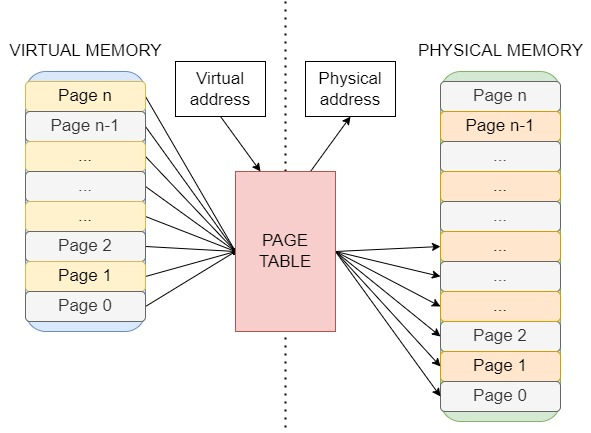
\includegraphics[width=13cm]{mem_arch_pages.jpg}
	\caption{Memory translation of virtual pages to physical pages.}
	\label{fig:mem_arch_pages}
\end{figure}

As we can observe in the figure, each virtual page is related to one physical page. However, RAM needs to maintain multiple processes and data simultaneously, and therefore sometimes the operating system (OS) will remove them from physical memory when it believes they are no longer being used. This leads to the occurrence of two type of memory events \cite{page_faults}:
\begin{itemize}
\item \textbf{Major page faults} occur when a process tries to access a virtual page, but the related physical page has been removed from RAM. In this case, the OS will need to request a secondary storage (such as a hard disk) for the data removed and allocate a new physical page for the virtual page. Figure \ref{fig:mem_major_page_fault} illustrates a major page fault.
\begin{figure}[htbp]
	\centering
	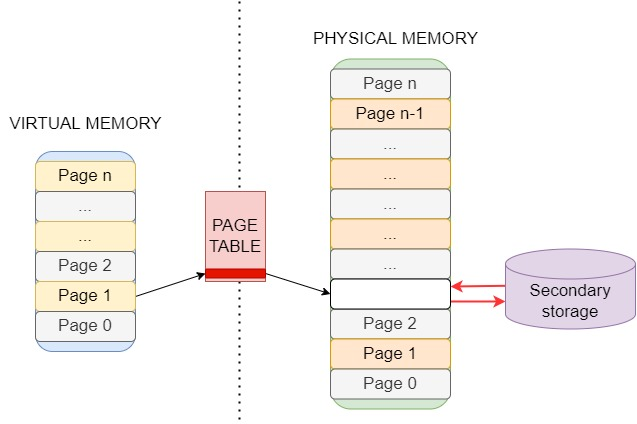
\includegraphics[width=11cm]{mem_major_page_fault.jpg}
	\caption{Major page fault after a page was removed from RAM.}
	\label{fig:mem_major_page_fault}
\end{figure}
\item \textbf{Minor page faults} occur when a process tries to access a virtual page, and although the related physical page exists, the connection in the page table has not been completed. A common event when these fault happen is on fork() calls, since with the purpose of making the call more efficient, the page table of the parent is not always completely copied into the child, leading into multiple minor page faults once the child tries to access the data on them. Figure \ref{fig:mem_minor_page_fault} illustrates a minor page fault after a fork.
\end{itemize}
\begin{figure}[htbp]
	\centering
	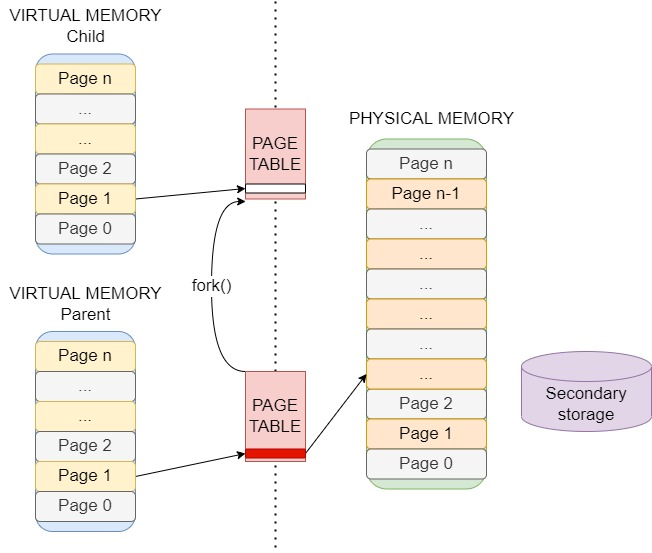
\includegraphics[width=11cm]{mem_minor_page_fault.jpg}
	\caption{Minor page fault after a fork() in which the page table was not copied completely.}
	\label{fig:mem_minor_page_fault}
\end{figure}

\subsection{Process virtual memory}
In the previous subsection we have studied that each process disposes of a virtual address space. We will now describe how this virtual memory is organized in a Linux system.

Figure \ref{fig:mem_proc_arch} describes how virtual memory is distributed within a process in the x86\_64 architecture. As we can observe, it is partitioned into multiple sections:
\begin{figure}[htbp]
	\centering
	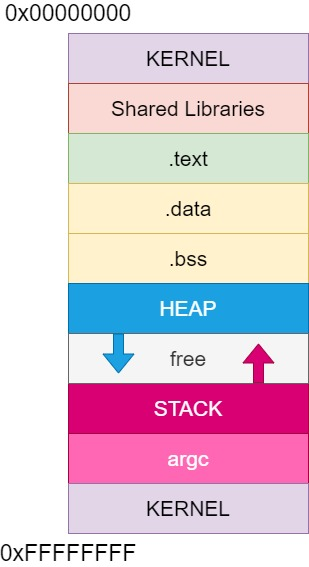
\includegraphics[width=6cm]{memory.jpg}
	\caption{Virtual memory architecture of a process \cite{mem_arch_proc}.}
	\label{fig:mem_proc_arch}
\end{figure}
\begin{itemize}
\item Lower and upper memory addresses are reserved for the kernel.
\item A section where shared libraries code is stored.
\item A .text section, which contains the code of the program being run.
\item A .data section, containing initialized static and global variables.
\item A .bss section, which contains global and static variables which are uninitialized or initialized to zero.
\item The heap, a section which grows from lower to higher memory addresses, and which contains memory dynamically allocated by the program.
\item The stack, a section which grows from higher to lower memory addresses, towards the heap. It is a Last In First Out (LIFO) structure used to store local variables, function parameters and return addresses.
\item Right at the start of the stack we can find the arguments with which the programs has been executed.
\end{itemize}

\subsection{The process stack} \label{subsection:stack}
Among all the sections we identified in a process virtual memory, the stack will be particularly relevant during our research. We will therefore study it now in detail. 

Firstly, we will present how the stack is structured, and which operations can be executed on it. Figure \ref{fig:stack_pres} presents a stack during the execution of a program. Table \ref{table:systemv_abi_other} explains the purpose of the most relevant registers related to the stack and program execution:

\begin{figure}[htbp]
	\centering
	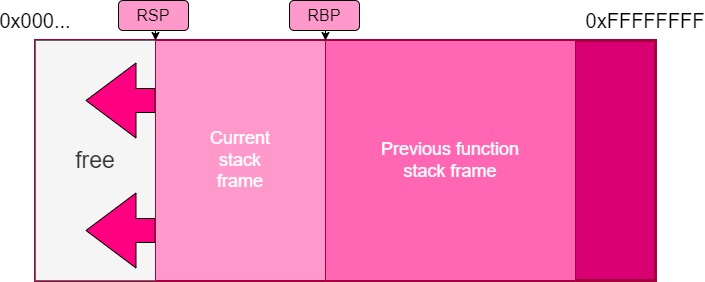
\includegraphics[width=14cm]{stack_pres.jpg}
	\caption{Simplified stack representation showing only stack frames.}
	\label{fig:stack_pres}
\end{figure}

\begin{table}[htbp]
\begin{tabular}{|>{\centering\arraybackslash}p{2cm}|>{\centering\arraybackslash}p{10cm}|}
\hline
\textbf{REGISTER} & \textbf{PURPOSE}\\
\hline
\hline
rip & Instruction Pointer - Memory address of the next instruction to execute\\
\hline
rsp & Stack Pointer - Memory address where next stack operation takes place\\
\hline
rbp & Base/Frame Pointer - Memory address of the start of the stack frame\\
\hline
\end{tabular}
\caption{Relevant registers in x86\_64 for the stack and control flow and their purpose.}
\label{table:systemv_abi_other}
\end{table}

As it can be observed in Figure \ref{fig:stack_pres}, the stack grows towards lower memory addresses, and it is organized in stack frames, delimited by the registers rsp and rbp. An stack frame is a division of the stack which contains all the data (variables, call arguments...) belonging to a single function execution. When a function is exited, its stack frame is removed, and if a function calls a nested function, then its stack frame is preserved and a new stack frame is inserted into the stack. 

As Table \ref{table:systemv_abi_other} explains, the rbp and rsp registers are used for keeping track of the starting and final position of the current stack frame respectively. We can see in Figure \ref{fig:stack_pres} that their value is a memory address pointing to their stack positions. On the other hand, the rip register does not point to the stack, but rather to the .text section (see Figure \ref{fig:mem_proc_arch}), where it points to the next instruction to be executed. However, as we will now see, its value must also be stored in the stack frame when a nested function is called, since after the nested function exits we need to restore the execution in the same instruction of the original function.

As with any LIFO structure, the stack supports two main operations: \textit{push} and \textit{pop}. In the x86\_64 architecture, it operates with chunks of data of either 16, 32 or 64 bytes. Table \ref{fig:stack_ops} shows a representation of these operations in the stack.
\begin{itemize}
\item A \textbf{push} operation writes data in the free memory pointed by register rsp. It then moves the value of rsp to point to the new end of the stack.
\item A \textbf{pop} operation moves the value of rsp by 16, 32 or 64 bytes, and reads the data previously saved in that position.
\end{itemize}

\begin{figure}[htbp]
	\centering
	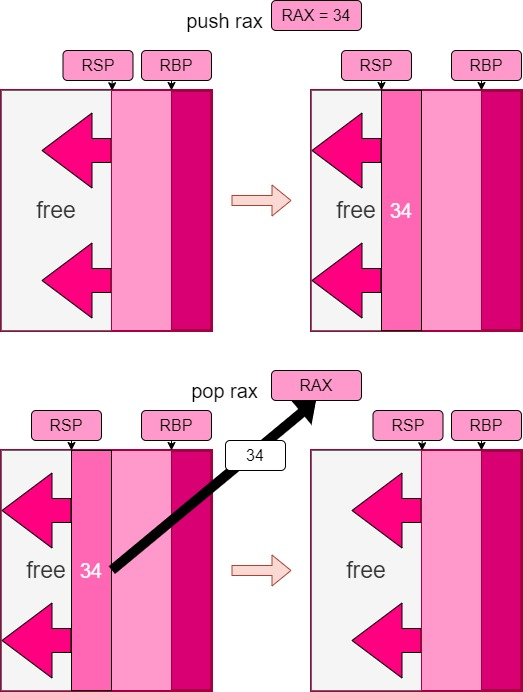
\includegraphics[width=10cm]{stack_ops.jpg}
	\caption{Representation of push and pop operations in the stack.}
	\label{fig:stack_ops}
\end{figure}


As we mentioned, the stack stores function parameters, return addresses and local variables inside a stack frame. We will now study how the processor uses the stack in order to call, execute, and exit a function. To illustrate this process, we will simulate the execution of function \lstinline{func(char* a, char* b, char* c)} \lstinline{}. Figures \ref{fig:stack_before} and \ref{fig:stack} show a representation of the stack during these operations.

\begin{figure}[htbp]
	\centering
	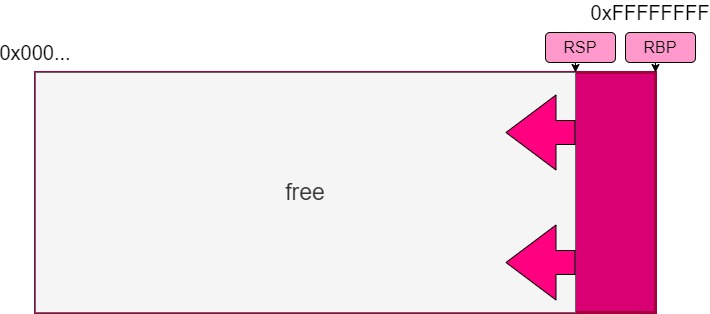
\includegraphics[width=14cm]{stack_before.jpg}
	\caption{Stack representation right before starting the function call process.}
	\label{fig:stack_before}
\end{figure}

\begin{figure}[htbp]
	\centering
	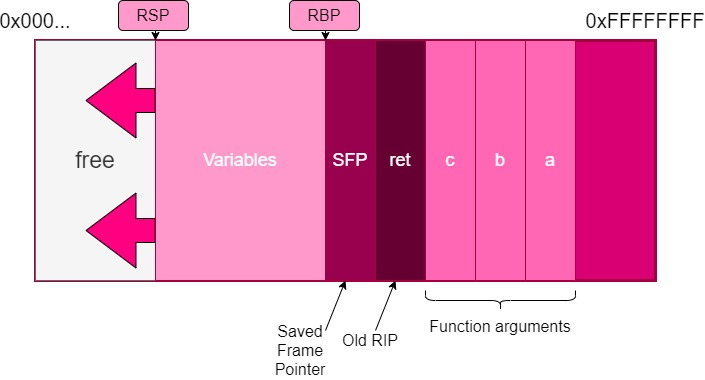
\includegraphics[width=14cm]{stack.jpg}
	\caption{Stack representation right after the function preamble.}
	\label{fig:stack}
\end{figure}

\begin{enumerate}
\item The function arguments are pushed into the stack. We can see them in the stack of Figure \ref{fig:stack} in reverse order. 
\item The function is called:
\begin{enumerate}
	\item The value of register rip is pushed into the stack, so that it is saved for when the function exists. We can see it on Figure \ref{fig:stack} as 'ret'.
	\item The value of rip changes to point to the first instruction of the called function.
\item We execute what is called as the \textit{function preamble} \cite{8664_params_abi_p18}, which prepares the stack frame for the called function:
\begin{enumerate}
	\item The value of rbp is pushed into the stack, so that we can restore the previous stack frame when the function exits. We can see it on Figure \ref{fig:stack} as the 'saved frame pointer'.
	\item The value of rsp is moved into rbp. Therefore, now rbp points to the end of the previous stack frame.
	\item The value of rsp is usually decremented (since the stack needs to go to lower memory addresses) so that we allocate some space for function variables.
\end{enumerate}
\end{enumerate}
\item The function instructions are executed. The stack may be further modified, but on its end rsp must point to the same address of the beginning. Register rbp always keeps pointing to the end of the stack.
\item We execute what is called the \textit{function epilogue}, which removes the stack frame and restores the original function:
\begin{enumerate}
	\item The value of rbp is moved into rsp, so that rsp points to the start of the previous stack frame. All data allocated in the previous stack frame is considered to be free.
	\item The value of the saved frame pointer is popped and stored into rbp, so that rbp now points to the start of the previous stack frame.
	\item The value of the saved rip value is popped into register rip, so that the next instruction to execute is the instruction right after the function call.
\end{enumerate}
\item Since the function arguments where pushed into the stack, they are popped now.
\end{enumerate}


\section{Attacks at the stack} \label{section:attacks_stack}
In Section \ref{subsection:stack}, we studied how the stack works and which is the process that a program follows in order to call a function. As we saw in Figure \ref{fig:stack}, the processor pushes into the stack several data which is used to restore the context of the original function once the called function exits. These pushed arguments included:
\begin{itemize}
\item The arguments with which the function is being called (if they need to be passed in the stack, such as byte arrays).
\item The original value of the rip register (ret), to restore the execution on the original function.
\item The original value of the rbp register (sfp), to restore the frame pointer of the original stack frame.
\end{itemize}

Although this process is simple enough, it opens the possibility for an attacker to easily hijack the flow of execution if it can modify the value of ret, as it is shown in figure \ref{fig:stack_ret_hij_simple}.
\begin{figure}[htbp]
	\centering
	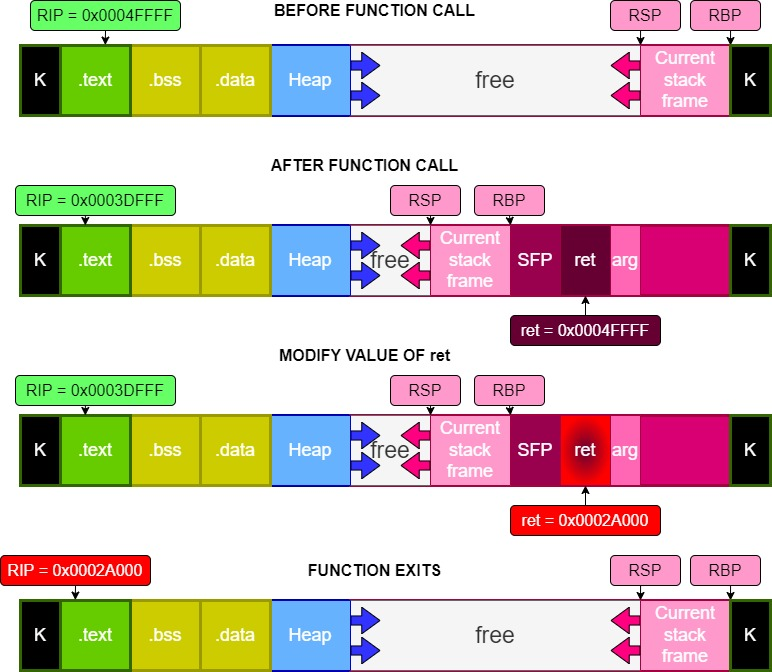
\includegraphics[width=15cm]{stack_ret_hij_simple.jpg}
	\caption{Execution hijack overwriting saved rip value.}
	\label{fig:stack_ret_hij_simple}
\end{figure}

In the Figure, we can observe how, during the execution of the called function, the attacker overwrites the value of ret in the stack. Once the function exists, as we explained in Section \ref{subsection:stack}, during the function epilogue the value of ret will be popped and moved into rip, so that the execution is directed to the original next instruction. However, because the value was modified, the attacker controls which instructions are executed next.

Attackers have historically used multiple techniques to overwrite the ret value in the stack. In this section, we will present two of the most popular techniques, which will be used as a basis for designing our own attacks using eBPF.

\subsection{Buffer overflow} \label{subsection: buf_overflow}
The stack buffer overflow is one of the most popular exploitation techniques to overwrite data at the stack. In this technique, an attacker takes advantage of a program receiving a user value stored in a buffer whose capacity is smaller of that of the supplied value. Code Snippet \ref{code:vuln_overflow} shows an example of a vulnerable program:

\begin{lstlisting}[language=C, caption={Program vulnerable to buffer overflow.}, label={code:vuln_overflow}]
void foo(char *bar){ // bar may be larger than 12 characters
   char buffer[12];
   strcpy(buffer, bar); //no bounds checking 
}

int main(int argc, char *argv[]){
   foo(argv[1]);
   return 0;
}
\end{lstlisting}

During the execution of the above program, since the char array \textit{buffer} is a buffer of length 12 stored in the stack, then if the value of \textit{bar} is larger than 12 bytes it will overflow the allocated space in the stack. This is usually the case of using unsafe functions for processing user input such as strcpy(), which do not check whether the array fits in the buffer. Figure \ref{fig:buffer_overflow} shows how the overflow happens in the stack.

\begin{figure}[htbp]
	\centering
	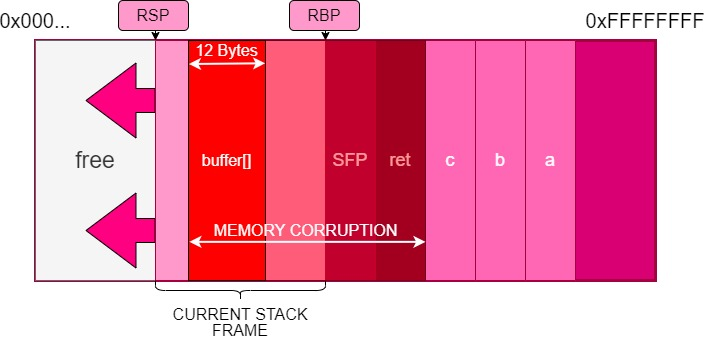
\includegraphics[width=15cm]{buffer_overflow.jpg}
	\caption{Stack buffer overflow overwriting ret value.}
	\label{fig:buffer_overflow}
\end{figure}

As we can observe in the figure, the new data written into the buffer has also overwritten other fields which were pushed into the stack, such as sfp and ret, resulting in changing the flow of execution once the function exists.

Usually, an attacker exploiting a program vulnerable to stack buffer overflow is interested in running arbitrary (malicious) code. For this, the attacker follows the process shown in Figure \ref{fig:buffer_overflow_shellcode}:

\begin{figure}[htbp]
	\centering
	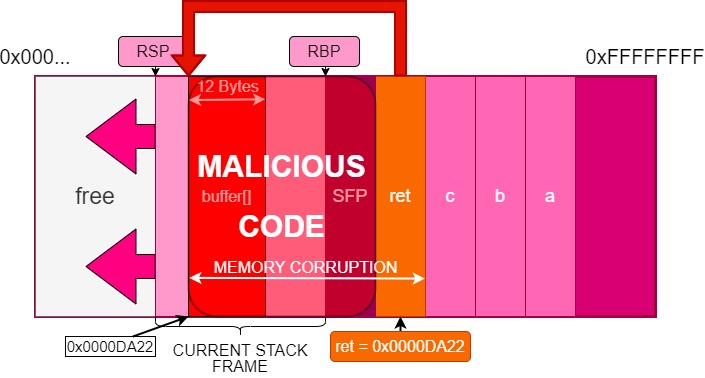
\includegraphics[width=15cm]{buffer_overflow_shellcode.jpg}
	\caption{Executing arbitrary code exploiting a buffer overflow vulnerability.}
	\label{fig:buffer_overflow_shellcode}
\end{figure}

As we can observe in the figure, the attacker will take advantage of the buffer overflow to overwrite not only ret, but also the rest of the current stack frame and sfp with malicious code. This code is known as shellcode, consisting of instruction opcodes (machine assembly instructions translated to their representation in hexadecimal values) which the processor will execute. We will explain how to write shellcode in Section \ref{subsection:got_attack}. Therefore, in this technique the attacker will:
\begin{itemize}
\item Introduce a byte array that overflows the buffer, consisting on SHELLCODE + the address of the buffer.
\begin{itemize}
	\item The shellcode overwrites the buffer and all data until ret.
	\item ret is overwritten by the value of the address where the buffer starts.
\end{itemize}
\item When the function exits and ret is popped from the stack, the register rip will now point to the address of the buffer at the stack, processing the stack data as instructions part of a program. The malicious code will be executed.
\end{itemize}

Although the classic buffer overflow is one of the best-known techniques in binary exploitation, it is also one of the oldest and thus numerous protections have historically been incorporated to mitigate this type of exploits. This is why the attack presented here does not work work in a modern system anymore. 

The reason is that one of the protections consists of the prohibition of executing code from the stack. By marking the stack as non-executable, in the case of rip pointing to an address in the stack any malicious code will not be run, even if an application was vulnerable to a buffer overflow. We will explain more in detail the main protections that nowadays are incorporated in modern systems in Section \ref{subsection:hardening_elf}.

\subsection{Return oriented programming attacks} \label{subsection:rop}
After the stack was marked non-executable, a new refined technique was invented to circumvent this restriction and adapt the classic buffer overflow to modern systems. In the end, attackers still maintained the ability to overflow the buffer in the stack of vulnerable applications, writing shellcode and overwriting ret, the only issue was that the shellcode could not be executed.

Return Oriented Programming (ROP) is an exploitation technique that takes advantage of the fact that, even if malicious code in the stack cannot be executed, the attacker can still redirect the flow of execution by modifying ret to any other piece of executable code. The challenge for the attacker is executing malicious code, since any available executable instructions are either at the .text section (which will correspond to the normal functioning of the program) or at shared libraries, but none are useful for malware. 

ROP tackles this challenge by designing a method of reconstructing malicious code from parts of already-existing code, as in a 'collage'. Assembly instructions are selected from multiple places, so that, when put together and executed sequentially, they recreate the shellcode which the attacker wants to execute. These pieces of code are called ROP gadgets, and consist of a set of arbitrary instructions followed by a final \textit{ret} instruction, which triggers the function exit and pops the value of ret. These gadgets may belong to any code in the process memory, usually selected between the code of the shared libraries (see Figure \ref{fig:stack}) to which the process is linked.

Finding ROP gadgets and writing ROP-compatible payloads manually is hard, thus multiple programs exist that automatically scan the system libraries and construct provide the gadgets given the shellcode to execute \cite{rop_prog_finder}.

However, we will now illustrate how ROP works with an example. Suppose that an attacker has discovered a buffer overflow vulnerability, but the stack is marked as not executable. The attacker wants to execute the assembly code shown in Code Snippet \ref{code:rop_ex}:

\begin{lstlisting}[language=C, caption={Sample program to run using ROP.}, label={code:rop_ex}]
mov rdx, 10
mov rax, [rsp]
\end{lstlisting}

After finding the address of the ROP gadgets manually or using an automated tool, the attacker takes advantage of a buffer overflow (or, in our case, a direct write using eBPF's bpf\_probe\_write\_user()) to overwrite the value of ret with the address of the first ROP gadget, and also additional data in the stack. Figure \ref{fig:rop_compund} shows how we can execute the original program using ROP:

\begin{figure}[htbp]
	\centering
	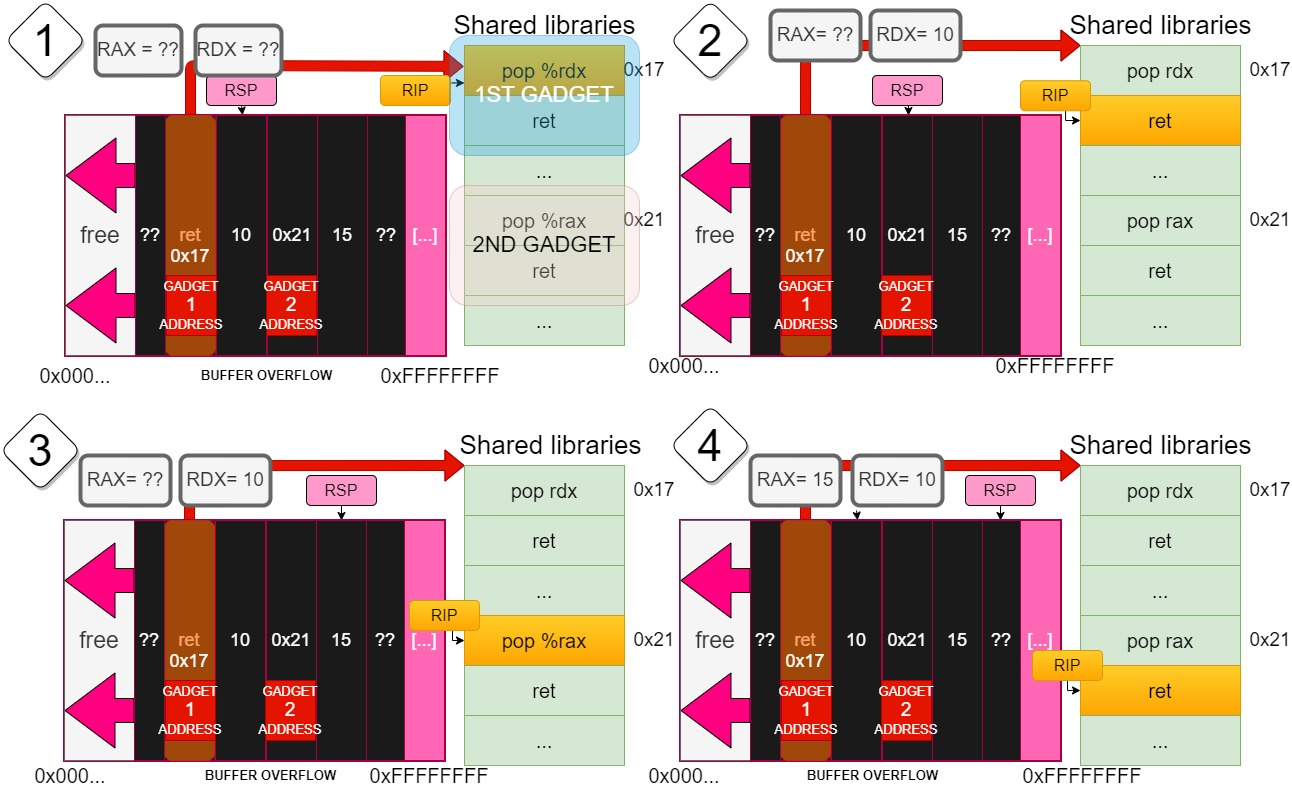
\includegraphics[width=15cm]{ROPcompound.jpg}
	\caption{Steps for executing code sample using ROP.}
	\label{fig:rop_compund}
\end{figure}

The steps described in the figure are the following:
\begin{enumerate}
\item First step shows the two gadgets located and their addresses, and the overwritten data in the stack. The function has already exited and, because ret was overwritten with the address of the first gadget, register rip now points to that location, and thus it is the next instruction to execute. Register rsp, in turn, now points to the bottom address of the current stack frame, which is right next to the old ret (see Section \ref{subsection:stack} for stack frames functioning).
\item The first instruction of the gadget is executed, popping the value from the stack (which also moves register rsp, see stack push and pop operations in Section \ref{subsection:stack}). As we can observe, the value "10" was specifically put in that position by the attacker, so that, according to the instruction to execute \lstinline{mov rdx, 10} \lstinline{}, we now have loaded that data into register rdx.
\item The return instruction is executed, which pops from the stack what is supposed to be the value of the saved rip, but in turn the attacker has placed the address of the next gadget there. Now, rip has jumped to the address of the second gadget. By continuing with this process, we can chain an infinite number of gadgets.
\item Finally, we repeated the same process as before, using a pop instruction to load a value from the stack. This illustrates that push and pop instructions, commonly used on most programs, are also possible to be using ROP.

After this step, the return instruction will be executed. Note that, at this point, if the attacker wants to be stealthy and avoid crashing the program (since we overwrote the original data in the stack), the original stack must be restored, together with the value of the registers before the malicious code execution. We will see an example of a technique for reconstructing the original state during our explanation of the library injection in Section \ref{subsection:got_attack}.
\end{enumerate}



\section{Networking fundamentals in Linux} \label{section:networking_fundamentals}
This section presents an overview on the most relevant aspects of the network system in Linux, which will be needed to tackle multiple of the techniques discussed during the design of the network capabilities of our rootkit. In particular, we will be focusing on the Ethernet, IP and TCP protocols.

\subsection{An overview on the network layer}
Firstly, we will describe the data structure we will be dealing with in networking programs. This will be Ethernet frames containing TCP/IP packets. Figure \ref{fig:frame} shows the frame in its completeness:

\begin{figure}[htbp]
	\centering
	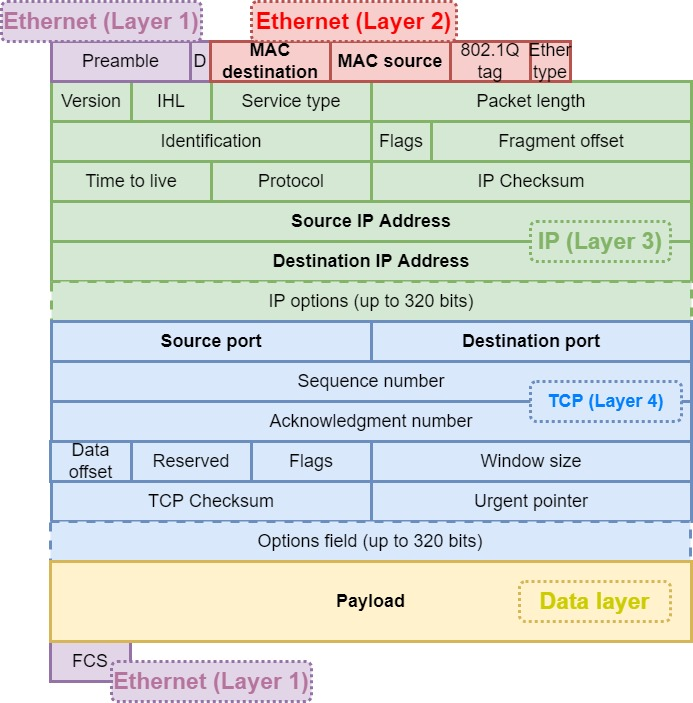
\includegraphics[width=14cm]{frame.jpg}
	\caption{Ethernet frame with TCP/IP packet.}
	\label{fig:frame}
\end{figure}

As we can observe, we can distinguish five different network layers in the frame. This division is made according to the OSI model \cite{network_layers}:
\begin{itemize}
\item Layer 1 corresponds to the physical layer, and it is processed by the NIC hardware, even before it reaches the XDP module (see Figure \ref{fig:xdp_diag}). Therefore, this layer is discarded and completely invisible to the kernel. Note that it does not only include a header, but also a trailer (a Frame Check Sequence, a redundancy check included to check frame integrity).
\item Layer 2 is the data layer, it is in charge of transporting the frame via physical media, in our case an Ethernet connection. Most relevant fields are the MAC destination and source, used for physical addressing.
\item Layer 3 is the network layer, in charge of packet forwarding and routing. In our case, packets will be using the IP protocol. Most relevant fields are the source and destination IP, used to indicate the host that sent the packet and who is the receiver.
\item Layer 4 is the transport layer, in charge of providing end-to-end connection services to applications in a host. We will be focusing on TCP during our research. Relevant fields include the source and destination port, which indicate the ports involved in the communication on which the applications on each host are listening and sending packets.
\item The last layer is the payload of the TCP packet, which contains, according to the OSI model, all layers belong to application data.
\end{itemize}


\subsection{Introduction to the TCP protocol} \label{subsection:tcp}
We will now focus our view on the transport layer, specifically on the TCP protocol, since it will be a major concern at the time of designing the network capabilities of our rootkit.

Firstly, since TCP aims to offer a reliable and ordered packet transmission \cite{tcp_reliable}, it includes sequence numbers (see Table \ref{fig:frame}) which mark the order in which they are transmitted. However, since the physical medium may corrupt or lose packets during the transmission, TCP must incorporate mechanisms for ensuring the order and delivery of all packets:
\begin{itemize}
\item Mechanism for opening and establishing a reliable connection between two parties.
\item Mechanism for ensuring that packets are retransmitted in case of an error during the connection.
\end{itemize}

With respect to the establishment of a reliable connection, this is achieved via a 3-way handshake, in which certain TCP flags will be set in a series of interchanged packets (see in Figure \ref{fig:frame} the field TCP flags). Most relevant TCP flags are described in Table \ref{table:tcp_flags}.

\begin{table}[htbp]
\begin{tabular}{|>{\centering\arraybackslash}p{3cm}|>{\centering\arraybackslash}p{10cm}|}
\hline
\textbf{FLAG} & \textbf{PURPOSE}\\
\hline
\hline
ACK & Acknowledges that a packet has been successfully received. In the acknowledgment number (see figure \ref{fig:frame}), it is stored the sequence number of the packet being acknowledged + 1. \\
\hline
SYN & Used during the 3-way handshake, indicates request for establishing a connection.\\
\hline
FIN & Used to request a connection termination.\\
\hline
RST & Abruptly terminates the connection, usually sent when a host receives an unexpected or unrecognized packet.\\
\hline
\end{tabular}
\caption{Relevant TCP flags and their purpose.}
\label{table:tcp_flags}
\end{table}

Taking the above into account, Figure \ref{fig:tcp_conn} shows a depiction of the 3-way handshake \cite{tcp_handshake}:
\begin{figure}[htbp]
	\centering
	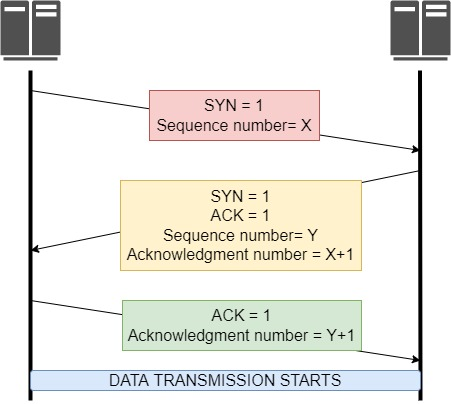
\includegraphics[width=12cm]{tcp_conn.jpg}
	\caption{TCP 3-way handshake.}
	\label{fig:tcp_conn}
\end{figure}

As we can observe in the figure, the hosts interchange a sequence of SYN, SYN+ACK, ACK packets, after which the communication starts. During this communication, the sender transmits packets with data (and no flags set), to which it expects an ACK packet acknowledging having received it.

With respect to maintaining the integrity of the connection once it starts, TCP works using timers, as it is illustrated in Figure \ref{fig:tcp_retransmission}:
\begin{enumerate}
\item A data packet with sequence number X is sent. The timer starts.
\item The destination host receives the packet and returns an ACK packet with acknowledgment number X+1.
\item The sender receives the ACK packet and stops the timer. If, for any reason, the ACK packet is not received before the timer ends, then the same packet is retransmitted.
\end{enumerate}

\begin{figure}[htbp]
	\centering
	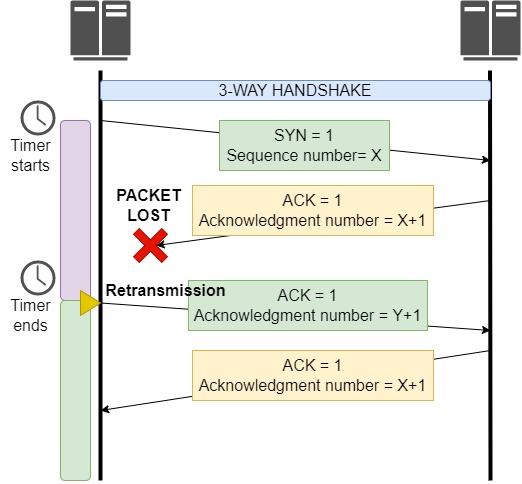
\includegraphics[width=12cm]{tcp_retransmission.jpg}
	\caption{TCP packet retransmission on timeout.}
	\label{fig:tcp_retransmission}
\end{figure}

\section{ELF binaries} \label{section:elf}
This section details the Executable and Linkable Format (ELF) \cite{elf}, the format in which we find executable files (between other file types) in Linux systems. We will perform an analysis from a security standpoint, that is, mainly oriented to describe the most relevant sections and the permissions incorporated into them. We will also focus on several of these sections which will be relevant for designing our attack.

After that, we will overview the security hardening techniques that have been historically incorporated into Linux to mitigate possible exploitation techniques when running ELF executables (such as the stack buffer overflow we explained in Section \ref{subsection: buf_overflow}). During the design of our rootkit, we will attempt to bypass these techniques using multiple workarounds.

\subsection{The ELF format and Lazy Binding} \label{subsection:elf_lazy_binding}
Linux supports multiple tools that enable a deep inspection of ELF binaries and its sections. Table \ref{table:elf_tools} shows the main tools we will use during this analysis:

\begin{table}[htbp]
\begin{tabular}{|>{\centering\arraybackslash}p{3cm}|>{\centering\arraybackslash}p{10cm}|}
\hline
\textbf{TOOL} & \textbf{PURPOSE}\\
\hline
\hline
Readelf & Display information about ELF files\\
\hline
Objdump & Display information about object files, mainly used for decompiling programs\\
\hline
GDB & The GNU Project Debugger, allows for debugging programs during runtime\\
\hline
GDB-peda & The Python Exploit Development Assistance for GDB, allows for multiple advanced operations that ease exploit development, such as showing register values, the stack state or memory information. It works as a plugin for GDB.\\
\hline
\end{tabular}
\caption{Tools used for analysis of ELF programs.}
\label{table:elf_tools}
\end{table}

Firstly, we will analyse the main sections we can find in an ELF executable. We will approach this study using a sample program that has been compiled using Clang/LLVM, and that consists on a simple timer that counts twice up to number 3, available at our repository \cite{repo_simple_timer}.

The commands used for this analysis and complete list of headers can be found in \nameref{annex:readelf_commands}. The most relevant sections we found at the program are described in Table \ref{table:elf_sec_headers}:

\begin{table}[htbp]
\begin{tabular}{|>{\centering\arraybackslash}p{1cm}|>{\centering\arraybackslash}p{9cm}|>{\centering\arraybackslash}p{2cm}|}
\hline
\textbf{TOOL} & \textbf{PURPOSE} & \textbf{PERMS}\\
\hline
\hline
.init & Contains instructions executed before the \textit{main} function of the program & Alloc, Executable\\
\hline
.plt & Procedure Linkage Table (PLT), contains code stubs that use the addresses at .got.plt for jumping to position-independent code & Alloc, Executable\\
\hline
.got & Global Offset Table (GOT), it contains addresses of global variables and functions once the linker resolves them at runtime & Alloc, Writable\\
\hline
.got.plt & A subset of .got section separated from .got with some compilers, it contains only the target addresses of position-independent code once the linker loads them at runtime, used by .plt section. & Alloc, Writable\\
\hline
.plt.got & Generated depending on compiler options, it is a PLT section which does not use lazy binding. & Alloc, Executable\\
\hline
.text & Stores executable instructions. & Alloc, Executable\\
\hline
.data & Contains initialized static and global variables. & Alloc, Writable\\
\hline
.bss & Contains global and static variables which are uninitialized or initialized to zero. & Alloc, Writable\\
\hline 
\end{tabular}
\caption{Sections in an ELF file.}
\label{table:elf_sec_headers}
\end{table}

As it can be observed in Table \ref{table:elf_sec_headers}, we can find that all sections have the Alloc flag, meaning they will be loaded into process memory during runtime.

Apart from those we have already discussed previously, we can find the GOT and PLT sections, whose purpose is to support Position Independent Code (PIC), that is, instructions whose address in virtual memory is not hardcoded by the compiler into the executable, but rather they are not known until resolved at runtime. This is usually the case of shared libraries, which can be loaded into virtual memory starting at any address \cite{plt_got_overlord}.

Therefore, in order to call a function of a shared library, the dynamic linker follows a process called 'Lazy binding' \cite{plt_got_technovelty}:
\begin{enumerate}
\item From the .text section, instead of calling a direct absolute address as usual, a PLT stub (in the .plt section) is called. Snippet \ref{code:lazy_bind_1} shows a call to the function timerfd\_settime, implemented by the shared library glibc and thus using a PLT.
\begin{lstlisting}[language=C, caption={Call to PLT stub seen from objdump.}, label={code:lazy_bind_1}]
$ objdump -d simple_timer
4014cb:	b9 00 00 00 00       	mov    $0x0,%ecx
4014d0:	be 01 00 00 00       	mov    $0x1,%esi
4014d5:	89 c7                	mov    %eax,%edi
4014d7:	e8 44 fc ff ff       	call   401120 <timerfd_settime@plt>
\end{lstlisting}

\item In the PLT stub, the flow of execution jumps to an address which is stored in the GOT section, which is the absolute address of the function at glibc. This address must be written there by the dynamic linker but, according to lazy binding, the first time to call this function the linker has not calculated that address yet. 

\begin{figure}[htbp]
	\centering
	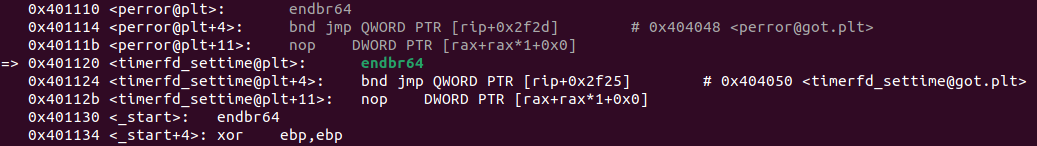
\includegraphics[width=14.5cm]{sch_gdb_plt.png}
	\caption{PLT stub for timerfd\_settime, seen from gdb-peda.}
	\label{fig:lazy_bind_2}
\end{figure}

\begin{figure}[htbp]
	\centering
	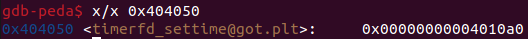
\includegraphics[width=14.5cm]{sch_gdb_got_prev.png}
	\caption{Inspecting address stored in GOT section before dynamic linking, seen from gdb-peda.}
	\label{fig:lazy_bind_3}
\end{figure}

\item As we can see in Figures \ref{fig:lazy_bind_2} and \ref{fig:lazy_bind_3}, the PLT stub calls address 0x4010a0, which leads to a dynamic linking routine, which proceeds to write the address into the GOT section and jump back to the start of the PLT stub. This time, the memory address at GOT to which the PLT jumps is already loaded with the address to the function at the shared library, as shown by Figure \ref{fig:lazy_bind_4}.

\begin{figure}[htbp]
	\centering
	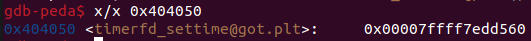
\includegraphics[width=14.5cm]{sch_gdb_got_after.png}
	\caption{Inspecting address stored in GOT section after dynamic linking, seen from gdb-peda.}
	\label{fig:lazy_bind_4}
\end{figure}

\begin{figure}[htbp]
	\centering
	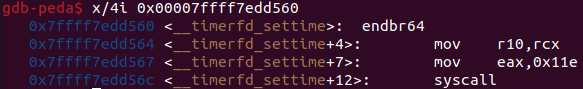
\includegraphics[width=14.5cm]{sch_glibc_func.png}
	\caption{Glibc function to which PLT jumps using address stored at GOT, seen from gdb-peda.}
	\label{fig:lazy_bind_5}
\end{figure}

\end{enumerate}

Therefore, in essence, when using lazy binding the dynamic linker will individually load into GOT the addresses of the functions at the shared libraries, during the first time they are called in the program. After that, the address will remain in the GOT section and will be used by the PLT for all subsequent calls.

The reason lazy binding matters to us is because, as we will explain Section \ref{subsection:got_attack}, the GOT section is actually writable from an eBPF program. This is because this section specifically must be writeable at runtime for the dynamic linker to store the address once they are resolved. Therefore, we would be able to modify the GOT section from eBPF, redirecting the address at which the PLT jumps, and thus controlling the flow of execution in the program. 

\subsection{Hardening ELF binaries} \label{subsection:hardening_elf}
During Section \ref{section:attacks_stack}, we presented multiple of the classic attacks at the stack such as buffer overflow and ROP. However, as we mentioned, during the years multiple hardening measures have been introduced into modern compilers, which attempt to mitigate these and other techniques. We will now present them so that, during the design of our rootkit, we can attempt to bypass all of these.

Table \ref{table:compilers} shows the compilers that we will be considering during this study. We will be exclusively looking at those security features that are included by default.

\begin{table}[htbp]
\begin{tabular}{|>{\centering\arraybackslash}p{5cm}|>{\centering\arraybackslash}p{9cm}|}
\hline
\textbf{COMPILER} & \textbf{SECURITY FEATURES BY DEFAULT}\\
\hline
\hline
Clang/LLVM 12.0.0 (2021) & Stack canaries, DEP/NX, ASLR\\
\hline
GCC 10.3.0 (2021) & Stack canaries, DEP/NX, ASLR, PIE, Full RELRO\\
\hline 
\end{tabular}
\caption{Security features in C compilers used in the study.}
\label{table:compilers}
\end{table}

\textbf{Stack canaries}\\
Stack canaries are random data that is pushed into the stack before calling potentially vulnerable functions (such as strcpy()) that attempts to prevent attacks at the stack by ensuring that their value is the same before and after the execution of the called function. It is particularly useful at detecting buffer overflow attacks.

If a stack canary is present and a buffer overflow happened, it would potentially overwrite the value of the canary, therefore alerting of the attack, in which case the processor halts the execution of the program.

\textbf{DEP/NX}\\
Data Execution Prevention, also known as No Execute, is the option of marking the stack as non-executable. This prevents, as we explained in Section \ref{subsection: buf_overflow}, the possibility of executing injected shellcode in the stack after modifying the value of the saved rip.

The creation of advanced techniques like ROP is one reaction to this mitigation, that circumvents this protection.

\textbf{ASLR}\\
Address Space Layout Randomization is a technique that randomizes the position of memory sections in a process virtual memory, including the heap, stack and libraries, so that an attacker cannot rely on known addresses during exploitation (e.g.: libraries are loaded at a different memory address each time the program is run, so ROP gadgets change their position) \cite{aslr_pie_intro}.

In the context of a stack buffer overflow attack, the memory position of the stack is random, and therefore even if shellcode is injected into the stack by an attacker, the address at which it resides cannot be written into the saved value of rip in order to hijack the flow of execution.

\textbf{PIE}\\
Position Independent Executable is a mitigation introduced to reduce the ability of an attacker to locate symbols in virtual memory by randomizing the base address at which the program itself (including the .text section) is loaded. This base address determines an offset which is added to all memory addresses in the code, so that each instruction is located at an address + this offset. Therefore, all jumps are made using relative addresses \cite{aslr_pie_intro}.

\textbf{RELRO}\\
Relocation Read-Only is a hardening technique that mitigates the possibility of an attacker overwriting the GOT section, as we explained at Section \ref{subsection:elf_lazy_binding}. In order to achieve the lazy binding process is substituted by the linker resolving all entries in the GOT section right after the beginning of the execution, and then marking the .got section as read-only. 

Two settings for RELRO are the most widespread, either Partial RELRO (which only marks sections of the .got section not related to the PLT as read-only, leaving .got.plt writeable) or Full RELRO (which marks the .got section as read-only completely). Binaries with only Partial RELRO are still non-secure, as the address at which the PLT section jumps can still be overwriten (including from eBPF, as we will explain) \cite{relro_redhat}.

\textbf{Intel CET}\\
Intel Control-flow Enforcement Technology is a hardening feature fully incorporated in Windows 10 systems \cite{cet_windows} and a work in progress in Linux \cite{cet_linux}. Its purpose is to defeat ROP attacks and other derivates (e.g: Jump-oriented programming, JOP), by adding a strict kernel-supported control of the return addresses and strong restrictions over jump and call instructions.

In Linux, the kernel will support a hidden 'shadow stack' that will save the return addresses for each call. This prevents modifying the saved value of rip in the stack, since the kernel would realise that the flow of execution has been modified. We can also find that modern compilers (such as GCC 10.3.0) already generate Intel CET-related instructions such as \textit{endbr64}, whose purpose is to be placed at the start of functions, marking that as the only address to which an indirect jump can land (otherwise, jumps will be rejected if not landing at \textit{endbr64}).

As mentioned, we will not consider this feature since it is not active in the Linux kernel.

\section{The proc filesystem} \label{section:proc_filesystem}
The proc filesystem is a virtual filesystem which provides an interface to kernel data structures \cite{proc_fs}. It can be found mounted automatically at \textit{/proc}.

This filesystem offers a great range of capabilities to interact with the kernel internal structures, however, in this section, we will focus on the most relevant files and directories for our research.

Specifically, we will be studying the files under the \textit{/proc/<pid>/} directory, whose purpose is to expose information about the process with the corresponding process ID.

Note that the access control for the \textit{/proc/<pid>/} is governed by the value set at \textit{/proc/sys/kernel/yama/ptrace\_scope}. Table \ref{table:yama_values} show its possible values.

\begin{table}[htbp]
\begin{tabular}{|>{\centering\arraybackslash}p{3cm}|>{\centering\arraybackslash}p{11cm}|}
\hline
\textbf{VALUE} & \textbf{DESCRIPTION}\\
\hline
\hline
0 & Unprivileged processes may access any file or subdirectory\\
\hline
1 & Only privileged processes or those belonging to that PID may access the any file. Unprivileged process can still list the directories at \textit{/proc}, finding the complete list of running processes.\\
\hline
2 & Only privileged processes or those belonging to that PID may access the any file. Unlike with setting '1', unprivileged users cannot list the directores at \textit{/proc} anymore.\\ 
\hline
\end{tabular}
\caption{Values for \textit{/proc/sys/kernel/yama/ptrace\_scope}.}
\label{table:yama_values}
\end{table}

In Ubuntu 21.04, the value of this setting is of '1', therefore the access is limited to users with root privileges or to unprivileged users accessing only their own or their children process information.

\subsection{/proc/<pid>/maps} \label{subsection:proc_maps}
This file provides, for the process with process ID <pid>, its mapped memory regions and their access permissions, that is, those virtual memory pages actively connected to a physical memory page (as shown in Figure \ref{fig:mem_arch_pages}).

Figure \ref{fig:proc_maps_sample} shows the maps file of a simple program. As we can observe, by reading this file we can get information such as:
\begin{itemize}
\item The virtual addresses that limit each memory section.
\item The permissions over each memory section.
\item In the case of memory from a file, the offset from which the data was loaded.
\item A pathname, in the case that memory section was loaded from a file.

The ability to easily find memory sections on the virtual address space of a process with a specific set of permissions is particularly relevant for this research. Also, apart from disclosing the address of the stack (and sometimes the heap too), we can infer the address of other memory sections such as the .text section, which must be the only one marked as executable (in Figure \ref{fig:proc_maps_sample}, the second entry that appears).

\end{itemize}

\begin{figure}[htbp]
	\centering
	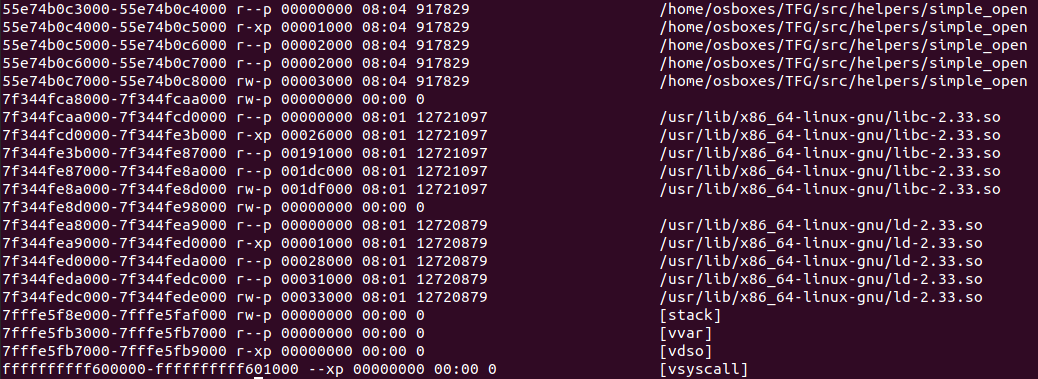
\includegraphics[width=15cm]{sch_proc_maps_sample.png}
	\caption{File /proc/<pid>/maps of a sample program.}
	\label{fig:proc_maps_sample}
\end{figure}

\subsection{/proc/<pid>/mem}
This file enables a process to access the virtual memory of the process with process id <pid>. According to the documentation, "this file can be used to access the pages of a process's memory through open(2), read(2), and lseek(2)" \cite{proc_fs}, meaning that we can read any memory address from the virtual memory space of the process.

However, we found the documentation not to be complete. In our experience, not only we can read virtual memory, but also freely write into it. There existed some discussions in the Linux community, and it was considered safe enough to be set as writeable by privileged programs \cite{proc_mem_write}, although the changes were never reflected in the official documentation.

Apart from being able to write into virtual memory, this write accesses are performed without regard of the permission flags set on each memory section. Therefore, we can modify non-writeable virtual memory by writing into the \textit{/proc/<pid>/mem} file.

